%%%%%%%%%%%%%%%%%%%%%%%%%%%%%%%%%%%%%%%%%%%%%%%%%%%%%%%%%%%%%%%
%% OXFORD THESIS TEMPLATE

% Use this template to produce a standard thesis that meets the Oxford University requirements for DPhil submission
%
% Originally by Keith A. Gillow (gillow@maths.ox.ac.uk), 1997
% Modified by Sam Evans (sam@samuelevansresearch.org), 2007
% Modified by John McManigle (john@oxfordechoes.com), 2015
% Modified by Ulrik Lyngs (ulrik.lyngs@cs.ox.ac.uk), 2018-, for use with R Markdown
%
% Ulrik Lyngs, 25 Nov 2018: Following John McManigle, broad permissions are granted to use, modify, and distribute this software
% as specified in the MIT License included in this distribution's LICENSE file.
%
% John commented this file extensively, so read through to see how to use the various options.  Remember that in LaTeX,
% any line starting with a % is NOT executed.  Several places below, you have a choice of which line to use
% out of multiple options (eg draft vs final, for PDF vs for binding, etc.)  When you pick one, add a % to the beginning of
% the lines you don't want.


%%%%% PAGE LAYOUT
% The most common choices should be below.  You can also do other things, like replacing "a4paper" with "letterpaper", etc.

% This one formats for two-sided binding (ie left and right pages have mirror margins; blank pages inserted where needed):
%\documentclass[a4paper,twoside]{templates/ociamthesis}
% This one formats for one-sided binding (ie left margin > right margin; no extra blank pages):
%\documentclass[a4paper]{ociamthesis}
% This one formats for PDF output (ie equal margins, no extra blank pages):
%\documentclass[a4paper,nobind]{templates/ociamthesis}

% As you can see from the uncommented line below, oxforddown template uses the a4paper size, 
% and passes in the binding option from the YAML header in index.Rmd:
\documentclass[a4paper, nobind]{templates/ociamthesis}


%%%%% ADDING LATEX PACKAGES
% add hyperref package with options from YAML %
\usepackage[pdfpagelabels]{hyperref}
% change the default coloring of links to something sensible
\usepackage{xcolor}

\definecolor{mylinkcolor}{RGB}{0,0,139}
\definecolor{myurlcolor}{RGB}{0,0,139}
\definecolor{mycitecolor}{RGB}{0,33,71}

\hypersetup{
  hidelinks,
  colorlinks,
  linktocpage=true,
  linkcolor=mylinkcolor,
  urlcolor=myurlcolor,
  citecolor=mycitecolor
}



% add float package to allow manual control of figure positioning %
\usepackage{float}

% enable strikethrough
\usepackage[normalem]{ulem}

% use soul package for correction highlighting
\usepackage{color, soul}
\definecolor{correctioncolor}{HTML}{CCCCFF}
\sethlcolor{correctioncolor}
\newcommand{\ctext}[3][RGB]{%
  \begingroup
  \definecolor{hlcolor}{#1}{#2}\sethlcolor{hlcolor}%
  \hl{#3}%
  \endgroup
}
\soulregister\ref7
\soulregister\cite7
\soulregister\autocite7
\soulregister\textcite7
\soulregister\pageref7

%%%%% FIXING / ADDING THINGS THAT'S SPECIAL TO R MARKDOWN'S USE OF LATEX TEMPLATES
% pandoc puts lists in 'tightlist' command when no space between bullet points in Rmd file,
% so we add this command to the template
\providecommand{\tightlist}{%
  \setlength{\itemsep}{0pt}\setlength{\parskip}{0pt}}
 
% UL 1 Dec 2018, fix to include code in shaded environments

% User-included things with header_includes or in_header will appear here
% kableExtra packages will appear here if you use library(kableExtra)
\usepackage{booktabs}
\usepackage{longtable}
\usepackage{array}
\usepackage{multirow}
\usepackage{wrapfig}
\usepackage{float}
\usepackage{colortbl}
\usepackage{pdflscape}
\usepackage{tabu}
\usepackage{threeparttable}
\usepackage{threeparttablex}
\usepackage[normalem]{ulem}
\usepackage{makecell}
\usepackage{xcolor}


%UL set section header spacing
\usepackage{titlesec}
% 
\titlespacing\subsubsection{0pt}{24pt plus 4pt minus 2pt}{0pt plus 2pt minus 2pt}


%UL set whitespace around verbatim environments
\usepackage{etoolbox}
\makeatletter
\preto{\@verbatim}{\topsep=0pt \partopsep=0pt }
\makeatother



%%%%%%% PAGE HEADERS AND FOOTERS %%%%%%%%%
\usepackage{fancyhdr}
\setlength{\headheight}{15pt}
\fancyhf{} % clear the header and footers
\pagestyle{fancy}
\renewcommand{\chaptermark}[1]{\markboth{\thechapter. #1}{\thechapter. #1}}
\renewcommand{\sectionmark}[1]{\markright{\thesection. #1}} 
\renewcommand{\headrulewidth}{0pt}

\fancyhead[LO]{\emph{\leftmark}} 
\fancyhead[RE]{\emph{\rightmark}} 

% UL page number position 
\fancyfoot[C]{\emph{\thepage}} %regular pages
\fancypagestyle{plain}{\fancyhf{}\fancyfoot[C]{\emph{\thepage}}} %chapter pages

% JEM fix header on cleared pages for openright
\def\cleardoublepage{\clearpage\if@twoside \ifodd\c@page\else
   \hbox{}
   \fancyfoot[C]{}
   \newpage
   \if@twocolumn\hbox{}\newpage
   \fi
   \fancyhead[LO]{\emph{\leftmark}} 
   \fancyhead[RE]{\emph{\rightmark}} 
   \fi\fi}


%%%%% SELECT YOUR DRAFT OPTIONS
% This adds a "DRAFT" footer to every normal page.  (The first page of each chapter is not a "normal" page.)

% IP feb 2021: option to include line numbers in PDF

% for line wrapping in code blocks
\usepackage{fvextra}
\DefineVerbatimEnvironment{Highlighting}{Verbatim}{breaklines,commandchars=\\\{\}}

% This highlights (in blue) corrections marked with (for words) \mccorrect{blah} or (for whole
% paragraphs) \begin{mccorrection} . . . \end{mccorrection}.  This can be useful for sending a PDF of
% your corrected thesis to your examiners for review.  Turn it off, and the blue disappears.
\correctionstrue


%%%%% BIBLIOGRAPHY SETUP
% Note that your bibliography will require some tweaking depending on your department, preferred format, etc.
% If you've not used LaTeX before, I recommend reading a little about biblatex/biber and getting started with it.
% If you're already a LaTeX pro and are used to natbib or something, modify as necessary.
% Either way, you'll have to choose and configure an appropriate bibliography format...


\usepackage[style=numeric-comp, sorting=none]{biblatex}
\newcommand*{\bibtitle}{References}

\addbibresource{bibliography/references.bib}
\addbibresource{bibliography/additional-references.bib}


% This makes the bibliography left-aligned (not 'justified') and slightly smaller font.
\renewcommand*{\bibfont}{\raggedright\small}


% Uncomment this if you want equation numbers per section (2.3.12), instead of per chapter (2.18):
%\numberwithin{equation}{subsection}


%%%%% THESIS / TITLE PAGE INFORMATION
% Everybody needs to complete the following:
\title{Dynamics of Learning Beyond Stochastic Gradient Descent\\}
\author{Doğan Can Demirbilek}
\college{}

% Master's candidates who require the alternate title page (with candidate number and word count)
% must also un-comment and complete the following three lines:

% Uncomment the following line if your degree also includes exams (eg most masters):
%\renewcommand{\submittedtext}{Submitted in partial completion of the}
% Your full degree name.  (But remember that DPhils aren't "in" anything.  They're just DPhils.)
\degree{Master in Data Science and Scientific Computing}
% Term and year of submission, or date if your board requires (eg most masters)
\degreedate{December 2021}


%%%%% YOUR OWN PERSONAL MACROS
% This is a good place to dump your own LaTeX macros as they come up.

% To make text superscripts shortcuts
	\renewcommand{\th}{\textsuperscript{th}} % ex: I won 4\th place
	\newcommand{\nd}{\textsuperscript{nd}}
	\renewcommand{\st}{\textsuperscript{st}}
	\newcommand{\rd}{\textsuperscript{rd}}

%%%%% THE ACTUAL DOCUMENT STARTS HERE
\begin{document}

%%%%% CHOOSE YOUR LINE SPACING HERE
% This is the official option.  Use it for your submission copy and library copy:
\setlength{\textbaselineskip}{22pt plus2pt}
% This is closer spacing (about 1.5-spaced) that you might prefer for your personal copies:
%\setlength{\textbaselineskip}{18pt plus2pt minus1pt}

% You can set the spacing here for the roman-numbered pages (acknowledgements, table of contents, etc.)
\setlength{\frontmatterbaselineskip}{17pt plus1pt minus1pt}

% UL: You can set the line and paragraph spacing here for the separate abstract page to be handed in to Examination schools
\setlength{\abstractseparatelineskip}{13pt plus1pt minus1pt}
\setlength{\abstractseparateparskip}{0pt plus 1pt}

% UL: You can set the general paragraph spacing here - I've set it to 2pt (was 0) so
% it's less claustrophobic
\setlength{\parskip}{2pt plus 1pt}

%
% Oxford University logo on title page
%
\def\crest{{
\includegraphics[width=5cm]{figures/logo.jpeg}}}
\renewcommand{\university}{University of Trieste}
\renewcommand{\submittedtext}{}


% Leave this line alone; it gets things started for the real document.
\setlength{\baselineskip}{\textbaselineskip}


%%%%% CHOOSE YOUR SECTION NUMBERING DEPTH HERE
% You have two choices.  First, how far down are sections numbered?  (Below that, they're named but
% don't get numbers.)  Second, what level of section appears in the table of contents?  These don't have
% to match: you can have numbered sections that don't show up in the ToC, or unnumbered sections that
% do.  Throughout, 0 = chapter; 1 = section; 2 = subsection; 3 = subsubsection, 4 = paragraph...

% The level that gets a number:
\setcounter{secnumdepth}{2}
% The level that shows up in the ToC:
\setcounter{tocdepth}{1}


%%%%% ABSTRACT SEPARATE
% This is used to create the separate, one-page abstract that you are required to hand into the Exam
% Schools.  You can comment it out to generate a PDF for printing or whatnot.

% JEM: Pages are roman numbered from here, though page numbers are invisible until ToC.  This is in
% keeping with most typesetting conventions.
\begin{romanpages}

% Title page is created here
\input{templates/alternative\_cover.tex}

%%%%% DEDICATION -- If you'd like one, un-comment the following.
\begin{dedication}
  \emph{To my family}
\end{dedication}

%%%%% ACKNOWLEDGEMENTS -- Nothing to do here except comment out if you don't want it.
\begin{acknowledgements}
 	This is where you will normally thank your advisor, colleagues, family and friends, as well as funding and institutional support. In our case, we will give our praises to the people who developed the ideas and tools that allow us to push open science a little step forward by writing plain-text, transparent, and reproducible theses in R Markdown.

We must be grateful to John Gruber for inventing the original version of Markdown, to John MacFarlane for creating Pandoc (\url{http://pandoc.org}) which converts Markdown to a large number of output formats, and to Yihui Xie for creating \texttt{knitr} which introduced R Markdown as a way of embedding code in Markdown documents, and \texttt{bookdown} which added tools for technical and longer-form writing.

Special thanks to \href{http://chester.rbind.io}{Chester Ismay}, who created the \texttt{thesisdown} package that helped many a PhD student write their theses in R Markdown. And a very special thanks to John McManigle, whose adaption of Sam Evans' adaptation of Keith Gillow's original maths template for writing an Oxford University DPhil thesis in LaTeX provided the template that I in turn adapted for R Markdown.

Finally, profuse thanks to JJ Allaire, the founder and CEO of \href{http://rstudio.com}{RStudio}, and Hadley Wickham, the mastermind of the tidyverse without whom we'd all just given up and done data science in Python instead. Thanks for making data science easier, more accessible, and more fun for us all.

\begin{flushright}
Ulrik Lyngs \\
Linacre College, Oxford \\
2 December 2018
\end{flushright}
\end{acknowledgements}


%%%%% ABSTRACT -- Nothing to do here except comment out if you don't want it.
\begin{abstract}
	This \emph{R Markdown} template is for writing an Oxford University thesis. The template is built using Yihui Xie's \texttt{bookdown} package, with heavy inspiration from Chester Ismay's \texttt{thesisdown} and the \texttt{OxThesis} \LaTeX~template (most recently adapted by John McManigle).

This template's sample content include illustrations of how to write a thesis in R Markdown, and largely follows the structure from \href{https://ulyngs.github.io/rmarkdown-workshop-2019/}{this R Markdown workshop}.

Congratulations for taking a step further into the lands of open, reproducible science by writing your thesis using a tool that allows you to transparently include tables and dynamically generated plots directly from the underlying data. Hip hooray!
\end{abstract}

%%%%% MINI TABLES
% This lays the groundwork for per-chapter, mini tables of contents.  Comment the following line
% (and remove \minitoc from the chapter files) if you don't want this.  Un-comment either of the
% next two lines if you want a per-chapter list of figures or tables.
  \dominitoc % include a mini table of contents

% This aligns the bottom of the text of each page.  It generally makes things look better.
\flushbottom

% This is where the whole-document ToC appears:
\tableofcontents

\listoffigures
	\mtcaddchapter
  	% \mtcaddchapter is needed when adding a non-chapter (but chapter-like) entity to avoid confusing minitoc

% Uncomment to generate a list of tables:
%%%%% LIST OF ABBREVIATIONS
% This example includes a list of abbreviations.  Look at text/abbreviations.tex to see how that file is
% formatted.  The template can handle any kind of list though, so this might be a good place for a
% glossary, etc.
% First parameter can be changed eg to "Glossary" or something.
% Second parameter is the max length of bold terms.
\begin{mclistof}{List of Abbreviations}{3.2cm}

\item[ANN]

Artificial Neural Network.

\item[BP]

Backpropagation.

\item[DFA]

Direct Feedback Alignment.

\item[BCE]

Binary Cross Entropy.

\item[FA]

Feedback Alignment.

\item[NTK]

Neural Tangent Kernel.

\item[t-SNE]

t-Distributed Stochastic Neighbor Embedding.

\item[SGD]

Stochastic Gradient Descent.

\item[NAG]

Nesterov Accelerated Gradient.

\end{mclistof} 


% The Roman pages, like the Roman Empire, must come to its inevitable close.
\end{romanpages}

%%%%% CHAPTERS
% Add or remove any chapters you'd like here, by file name (excluding '.tex'):
\flushbottom

% all your chapters and appendices will appear here
\hypertarget{introduction}{%
\chapter*{Introduction}\label{introduction}}
\addcontentsline{toc}{chapter}{Introduction}

\adjustmtc
\markboth{Introduction}{}

Artificial neural networks (ANNs) are a collection of connected computational nodes inspired by biological neural networks. Each connection can transmit a helpful signal to another computational node like synapses in a brain. ANNs demonstrated colossal advancements in the last decades. Thanks to these advancements, it is possible to solve complex problems in computer vision, speech recognition, and natural language processing within a reasonable amount of time and with satisfactory performance. These advancements were actualized through an old but robust algorithm called backpropagation (BP). BP is a training algorithm for ANNs based on repeatedly adjusting network weights to minimize the difference (loss) between the output of the network and the ground truth \cite{Rumelhart:1986we}.\\
Although nowadays BP is the workhorse algorithm for training ANNs, it has some drawbacks, and it is not the only alternative. Recent studies offered different algorithms to train ANNs by addressing these drawbacks. These algorithms have other properties and principles than BP. Some of them are competitive with BP, or they even outperform the BP in terms of performance or convergence speed for specific problems.\\
This thesis investigates the learning structures through BP and one of the alternative algorithm called direct feedback alignment (DFA) on the particular problem. Unlike BP, the error is propagated through a fixed random matrix instead of the layers' weights in DFA. Then network learns how to make this feedback useful \cite{nøkland2016direct}. Due to this error propagation mechanism, DFA is considered more biologically plausible than BP, and it opens the gate of parallelism in the training phase of ANNs.\\
The main problem at hand is known as the parity learning problem. Previous results showed that these parities are learnable by BP and lazy methods in a more simple setting, whereas it is only learnable by BP in a more complex setting \cite{DBLP:journals/corr/abs-2002-07400}. That is why it is intriguing to test alternative algorithms on this problem to understand their learning dynamics and capabilities.\\
The experiment results might lead us to three possible outcomes. First, we might acquire a similar performance as BP. If it is the case, it would be beneficial to test DFA and BP on a more challenging problem. Second, there might be a gap between BP and DFA then it would be intriguing to understand where the difference is coming from and how we can close this gap. Third, the alternative algorithm might not even learn, and in this case, it is interesting to ask what makes a problem learnable by BP but not DFA. In all cases, results should help to understand the dynamics of learning of both methods.\\
For applying BP and DFA in a more realistic setting, experiments are performed on the MNIST dataset by imitating the parity learning problem. After putting DFA to this frame, the reason behind the results is interpreted, and possible improvements are motivated and implemented.\\
Chapter \ref{chap:chapter_1} constructs the theoretical bases of the algorithms that are used for the experiments. These bases are composed of simple definitions, mathematical foundations, and the drawbacks of the algorithms. They help to dig deeper into the learning structures of the training algorithms. It is expected to have more control over their learning behaviors by adjusting components of these foundations. Also, it is beneficial to have these theoretical bases for acquiring a better understanding of the further interventions. Moreover, these theoretical foundations are used to implement the algorithms from scratch to use in experiments.\\
Chapter \ref{chap:chapter_2} introduces the parity learning problem at hand. First, the formal definition of the problem is demonstrated then how the problem is imitated by using the MNIST dataset is explained in detail. This part is also highly correlated with the training phase of the algorithms. Later experiment results from \cite{DBLP:journals/corr/abs-2002-07400} are replicated to have a concrete picture of previous studies.\\
Chapter \ref{chap:chapter_3} presents results of the experiments. This chapter is the main contribution of the study. The first experiment is testing DFA on the same problem and observing the difference with BP. As it is specified before, depending on the experiment outcome, different further experiments are performed. Such as closing the gap between BP and DFA, if any, trying harder problems if we acquire similar results. Explain why DFA cannot learn the problem if we get a similar behavior as lazy methods. In addition to the main experiment, we performed side experiments that helped us understand the algorithms' learning dynamics. For instance, using different random matrices for DFA, comparing their results, and observing hidden representation of BP and DFA to understand if the networks learn the digits individually to calculate the parities or memorizes the data without knowing the digits.\\
Chapter \ref{chap:chapter_4} wraps up the findings from experiments by summarizing the key findings. It creates a path for future studies that are not covered in this study.

\hypertarget{chap:chapter_1}{%
\chapter{Theoretical Foundations}\label{chap:chapter_1}}

\minitoc 

\hypertarget{backpropagation}{%
\section{Backpropagation}\label{backpropagation}}

BP is one of the first algorithms that show ANNs could learn hidden representations well. Numerous studies showed that ANNs trained with BP could capture similar information as biological neural networks (e.g., specific nodes learn the edges, corners). We need three components for BP, a dataset composed of input-output pairs, a network consisting of parameters (weights and biases), and it allows the input to flow through the network to have output. We need a loss function to measure the difference between the output of the network and the ground truth that we have from the dataset.\\
The main goal of BP is computing the gradients of the loss function (a measure of difference) concerning the parameters of neural networks by using the chain rule. These gradients show how much the parameter needs to change (positively or negatively) to minimize the loss function. After efficiently calculating the gradients, we can adjust the network parameters using gradient descent or its variants.\\
Although BP is an older idea, it earned popularity with \cite{Rumelhart:1986we} because it presented how BP can make a network to learn the representations. After this popularity, the community published numerous practical and theoretical papers that investigated the dynamics of BP. It would be repeat and infeasible to show all the aspects again. However, for completeness and a smoother transition from BP to DFA, it is beneficial to have visual and mathematical explanations showing how the algorithms propagate the errors and the weights. For the mathematical foundations, a binary classification task will be demonstrated with binary cross-entropy loss as an example in appendix \ref{chap:appendix_a}. This example is not chosen arbitrarily. Indeed the parity problem that MNIST imitates is a binary classification problem. In addition to this, equations from appendix \ref{chap:appendix_a} are used to implement BP from scratch to have more control over the process. Then the exact implementation is modified to obtain DFA. The same set of steps are valid for different loss functions and activation functions. Only the calculations will be slightly different. The general idea is the same: obtaining the gradients by calculating the derivative of the loss function concerning the parameters.

\begin{figure}

{\centering 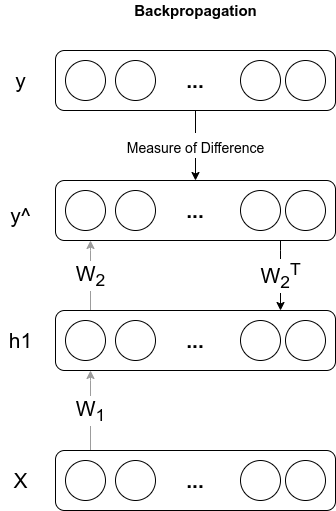
\includegraphics[width=0.3\linewidth]{figures/BP} 

}

\caption{Error Transportation in BP}\label{fig:BP-Error}
\end{figure}

\noindent In figure \ref{fig:BP-Error} we have a simple network with only a hidden layer that shows the error transportation configuration in BP. \(W_i\) are the weights, \(h_i\) are the output of the hidden layers that is denoted as \(i\), \(\hat{y}\) is the output of the network, and \(y\) is the ground truth, for the sake of simplicity, biases are not showed in this figure. It is important to note that in BP, the transpose of weight is propagated to calculate the gradients. In literature, this issue is known as the weight transport problem, and it is one of the most criticized disadvantages of BP.

\hypertarget{drawbacks-of-bp}{%
\subsection{Drawbacks of BP}\label{drawbacks-of-bp}}

We know that biological neurons inspired ANNs. However, recent studies showed that BP is not precisely how biological neurons learn \cite{bengio2016biologically}. This brings a term called biological plausibility of an algorithm that indicates the algorithm's consistency with existing biological, medical, and neuroscientific knowledge. That is why the community proposed many alternative algorithms by addressing these limitations of BP. In the light of this term, we can put in order the drawbacks of BP as the following:

\begin{itemize}
    \item \textbf{Biological implausibility:}
    \begin{itemize}
        \item The BP computation is purely linear whereas biological neurons interleave linear and non-linear operations.
        \item BP needs precise knowledge of derivatives of the non-linearities at the operating point used in the corresponding feedforward computation on the feedforward path.
        \item BP has to use exact symmetric weights of the feedforward connections.
        \item Real neurons communicate by binary values (spikes), not by clean continuous values.
        \item The computation has to be precisely clocked to alternate between feedforward and BP phases.
        \item It is not clear where the output targets would come from.
        \cite{bengio2016biologically, lee2015difference} 
    \end{itemize}  
    \item \textbf{Vanishing or Exploding Gradients}
    \item \textbf{Lack of Parallel Processing} \cite{ma2019hsic}
\end{itemize}

\noindent Simple interventions may handle some of these drawbacks. For instance, implementing gradient clipping or different activation functions might solve exploding gradients and vanishing gradients. However, they may frequently happen in deeper networks, and they must be considered while training ANNs. On the other hand, some of the drawbacks can not be handled with superficial modifications. For instance, BP is a sequential process, and there are locking mechanisms (forward, backward and update) that ensure none of the processes is executed before its preceding completion. This makes BP infeasible for parallel processing because each execution has to wait for its preceding process. Hence deeper and larger networks' training can be computationally expensive.\\
Biological plausibility is significant because of a couple of reasons. We know that biological neurons inspired ANNs, and biological plausibility refers to consistency between BP and biological knowledge about the neurons of a brain. Hence, it is interesting to examine the dissimilarity or similarity among them. Besides, there is a field that is the intersection of neuroscience and deep learning, so it is natural to investigate the biological plausibility feature of the algorithms, especially for this field. Furthermore, even though nowadays ANNs might outperform the human brain in a specific task, we are still distant from fully mimicking it. In other words, most of the time, ANNs are very good on a task that they are trained in, but they are not diverse, and some kinds of attacks like adversarial ones can easily trick them. Investigating the learning dynamics of these algorithms may open the doors of diverse ANNs that are not specialized in a single task or make them more robust to attacks.\\
Alternative algorithms address some of the drawbacks of BP, and they propose a solution to them, but they also demonstrate a couple of them. However, these algorithms can be considered one or more steps closer to more biologically plausible and robust algorithms.

\hypertarget{direct-feedback-alignment}{%
\section{Direct Feedback Alignment}\label{direct-feedback-alignment}}

So far, we have seen how the error is propagated in BP sequentially through a network with the backward pass. Unlike BP, DFA uses a different way to propagate the error. This way uses a random matrix instead of the transpose of the weight matrix, which brings a solution to the weight transport problem. Before explaining how DFA works, it is better to investigate the feedback alignment (FA) algorithm since DFA is the extension of FA.\\
In \cite{lillicrap2014random}, authors proved that precise symmetric weights are not required to obtain learning in ANNs. Without these matrices, BP-like learning can be obtained. Any random matrix under some conditions can provide the learning. Implicit dynamics in the standard forward weight updates encourage an alignment between weights and the random matrix. In other words, a random matrix pushes the network in roughly the same direction as BP would. They supported this hypothesis with some experiments on a linear problem and MNIST classification task. The empirical results demonstrate that FA successfully trains the network and has similar performance results as BP on these tasks.\\
Even though learning still occurs with random matrix and FA offers the solution to the weight transport problem, it does not provide any computational advantage. To extend DFA, we need to change the error propagation mechanism of FA slightly. In FA, the error is propagated through a random matrix, but the backward process is still sequential. DFA extends this idea and propagates the random matrix in parallel to each layer. In other words, DFA takes the loss and distribute it globally to all layers without requiring sequential step. It also creates an opportunity to parallelize the computation that might speed up the training process.

\begin{figure}

{\centering 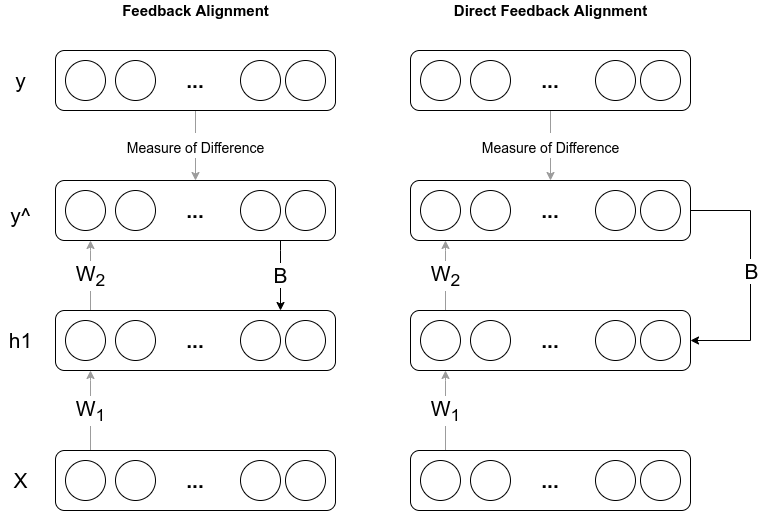
\includegraphics[width=0.65\linewidth]{figures/DFA} 

}

\caption{Error Transportation in DFA}\label{fig:DFA-Error}
\end{figure}

\noindent In figure \ref{fig:DFA-Error} we can see the error transportation configurations for FA and DFA. This figure is the same as the one in \cite{nøkland2016direct} but shows only one hidden layer. In fact, with only one hidden layer, FA and DFA are identical.\\
It is crucial to point out, BP and DFA have different learning dynamics. BP calculates the gradients that point to the steepest descent in the loss function space. On the other hand, FA and DFA provide a different update direction but still descending. It is still descending because empirical and theoretical results proved that the networks' weights align with the random matrix that leads to gradients alignment. Therefore the more alignment we have, the same direction would FA and DFA point as BP. Even though they have different update directions, since they are both descending, the results from \cite{lillicrap2014random, nøkland2016direct} showed that FA and DFA are as good as BP in terms of performance for specified tasks in these papers. In addition to this, ANNs trained with DFA show decent separation for labels as in BP's hidden representations of the layers. We can observe this from the t-distributed stochastic neighbor embedding (t-SNE) visualizations of the hidden layers' representations \cite{nøkland2016direct}. t-SNE is a method visualizing high-dimensional data which tries to keep the neighbor property in lower dimensions \cite{vanDerMaaten2008}.\\
Recently, a new study has been published which tests the applicability of DFA on modern deep learning tasks and architectures such as neural view synthesis, recommender systems, geometric learning, and natural language processing \cite{launay2020direct}. Because even though some of the alternative methods are competitive with BP in simple tasks like MNIST, they are not competitive or trainable on more complex tasks. Results showed that DFA successfully trains all these complex architectures with performance close to BP. This study supports that complex tasks can be solved without symmetric weight transport, proving that DFA is suitable for more challenging problems.\\
Let us use the same example as \ref{chap:appendix_a} to present how gradients are calculated in DFA. After having the mathematical foundations of BP, transition to DFA is relatively easy. The forward pass is the same as BP, whereas, in the backward pass, we need to replace the transpose of the weight matrix, which is used to calculate the gradients with the random matrix. Considering the same example, we have a simple binary classification task with binary cross-entropy loss, and our network has only one hidden layer. In this setting, gradients of the weights can be calculated as the following:
\[
\frac{\partial BCE}{\partial w_{2}}=h_{1}^T\left(\hat{y}-y\right)
\]
There is no change in the calculations of gradients of the last layer, whereas, for the hidden layer, we have:
\[
\begin{aligned}
\frac{\partial BCE}{\partial w_{1}}= \left(X\right)^T\left(\hat{y}-y\right)\left(B\right) \odot f'(a_1)
\end{aligned}
\]
Please pay attention that \(w_2^T\) is replaced with the random matrix \(B\). This means that we can obtain learning by changing either the random matrix or weight matrix. We know that in DFA, \(B\) is fixed, so the feedforward weights of the network will learn to make these signals useful by aligning with the BP's teaching signal.\\
Update rules are the same as BP, which means that gradient descent and its variants can be used.
\[
\begin{aligned} 
\text{parameter} &= \text{parameter} - \text{step size} \times \frac{\partial BCE}{\partial \text(parameter)}  \\
\end{aligned}
\]
With this tiny modification, DFA brings a solution to some of the drawbacks of BP. Such as using exact symmetric weights of the feedforward connections (weight transport problem), lack of parallel processing (random matrix can be propagated in parallel), and it is less likely to suffer from vanishing or exploding gradients than BP. Eventually, it proposes a more biologically plausible training method. However, it is not the perfect solution either. Because it assumes there is a global feedback path to propagate the error that might be biologically implausible because feedback has to travel a long physical distance. It also suffers some of the drawbacks of BP. For instance, computation is still purely linear. We still need precise knowledge of derivatives of non-linearities. We still communicate by clean, continuous values, and it is unclear where the output targets would come from. Besides, DFA has an extra task to accomplish while training the ANN that aligns with BP's weights, and a layer can not learn before its preceding layers are aligned. This might spawn performance concerns, and DFA might lag behind BP.
Furthermore, DFA fails to train convolutional neural networks which dominate the computer vision tasks \cite{refinetti2021align, launay2019principled}. Finally, unlike BP, DFA was not investigated on particular subjects like adversarial attacks and interpretability by the community. This leaves some question marks about the robustness of DFA.

\hypertarget{lazy-methods}{%
\section{Lazy Methods}\label{lazy-methods}}

Theoretical results present that especially over-parameterized ANNs (not limited to these networks) trained with gradient-based methods can reach zero training loss with their parameters barely changing. The term lazy does not refer to the poor property of methods, whereas they are called lazy methods because their parameters hardly move during training \cite{chizat2020lazy}.\\
Lazy methods are not at the center of the experiments. Hence, detailed explanations of these methods are out of scope in this study, but they have been presented in \cite{DBLP:journals/corr/abs-2002-07400}, and they fail to learn the parities in a more complex setting. Hence, they are implemented too for completeness, and it is essential to embody at least a simple definition of them and how they are practically implemented.

\hypertarget{neural-tangent-kernel}{%
\subsection{Neural Tangent Kernel}\label{neural-tangent-kernel}}

Studies showed that neural networks under some conditions are equivalent to gaussian process, and they mathematically approximate the kernel machines if they are trained with gradient descent \cite{lee2018deep, domingos2020model}. Authors of \cite{DBLP:journals/corr/abs-1806-07572} proved that during the training phase, ANNs follow the kernel gradient of the functional loss concerning a new kernel. They named this kernel a Neural Tangent Kernel (NTK). In other words, NTK is a kernel that describes the evolution of an ANN during the learning phase, and it is beneficial to explain the training of ANNs in function space rather than parameters space. It allows us to work with infinite width neural networks using the kernel trick, and it helps us understand the dynamics of learning and inference.\\
Empirical results demonstrated that the NTK regime performs worse than BP on standard tasks like MNIST. However, NTK is still worth investigating further to understand ANNs' training dynamics since it brings a new perspective on the training phase.\\
Basic practical implementation of NTK is obtained with three steps. Initially, an extra layer is created with the exact dimensions of the first layer. The second in the forward pass concatenation of these two layers' parameters are given as input to the gated linear unit with \(1\). Lastly, in the parameters update phase, the extra layer is not considered. With these adjustments, we decoupled the gating from the linearity of the ReLU, and we kept the gates fixed during training.

\hypertarget{random-features}{%
\subsection{Random features}\label{random-features}}

Standard random features are where first layer weights are initialized randomly by following a distribution and the train only the second layer. These mechanisms are particularly good at approximating kernels. They are preferred because kernel machines might take too much time to train if the data size is big. In \textbf{gaussian features} case, we initialize the first layer weights using gaussian distribution. In contrast, in \textbf{ReLU features} and \textbf{linear features}, we initialize the first layer weights uniformly but, for linear features, non-linear activation functions are not used in the forward pass.

\hypertarget{optimizers}{%
\section{Optimizers}\label{optimizers}}

Up to this point, we only mentioned how we could use gradient descent and its variants to update the weights of a network superficially. This part is worth further investigation because many variants provide better convergence properties to find the minimum of the loss function. We may take advantage of these methods to have better performance or faster convergence for BP and DFA. These methods may spawn a significant impact on convergence speed and overall performance. As a reference to the following methods, mostly \cite{DBLP:journals/corr/Ruder16} is used, also the structure of this part and mathematical notations are adapted from the same paper, it is an excellent overview for the optimizers, and it reviews their advantages as well as drawbacks.

\hypertarget{gradient-descent}{%
\subsection{Gradient Descent}\label{gradient-descent}}

Gradient descent is a first-order iterative optimization algorithm. It is the most used algorithm to optimize neural networks. It has three variants that depend on how much data we use to compute the gradients. \textbf{Batch gradient descent} computes the gradients for the entire dataset and performs only one update. \textbf{Stochastic gradient descent} (SGD), in contrast, calculates gradients for each training example and performs parameter update for each of them. Lastly, \textbf{mini-batch gradient descent} calculates the gradients of mini-batches and performs updates for each mini-batches.
Gradient descent is infeasible to implement for the datasets that do not fit in the memory. In contrast, SGD performs too frequent updates, spawning high variance in parameters that cause fluctuation in the loss function. SGD provides the same convergence properties as batch gradient descent if the learning rate periodically decreases through iterations. For our experiments, we used mini-batch gradient descent, which takes the best of two methods. Most of the implementations use SGD term instead of mini-batch gradient descent. The same tradition will be followed in this study too. Update rule of mini-batch gradient descent is the following:
\[
\theta_{t+1}=\theta_t-\eta \cdot \nabla_{\theta} J\left(\theta ; x^{(i: i+n)} ; y^{(i: i+n)}\right)
\]
where \(\theta\) is the parameters of the network, \(\eta\) is the learning rate or step size, \(\nabla_{\theta}\) is the gradients of the parameters and \(J\left(\theta ; x^{(i: i+n)} ; y^{(i: i+n)}\right)\) is the loss function for mini-batch \(i\) to \(i+n\).\\
There are a couple of challenges in SGD because it doesn't always guarantee good convergence:

\begin{itemize}
  \item Choosing a proper learning rate is intricate. Small learning rates may take too long to converge, whereas big learning rates may spawn loss function fluctuations and even diverge.
  \item SGD does not guarantee the global minimum. It can easily be stuck in the local minimum for highly non-convex loss functions that are standard for deep learning tasks.
  \item Same learning rate is applied to all parameters, but we may want to update the parameter by their frequencies.
  \item Convergence is strongly dependent on where the initial step starts. Unfortunate initializations may never reach the global minimum. 
\end{itemize}

\hypertarget{momentum}{%
\subsubsection{Momentum}\label{momentum}}

\noindent SGD has difficulties finding the direction in valleys because the gradients on these areas will be either zero or very close to zero, so it will slow down and make hesitant progress. These areas are prevalent around the local minimum. Momentum is an idea that dampens the oscillations in the relevant direction. It is accomplished by adding a fraction \(\gamma\) of the update vector of the past time step. This fraction is usually set to \(0.9\). This term usually leads to faster convergence and speeds up the iterations.
\[
\begin{aligned}
v_{t} &=\gamma v_{t-1}+\eta \nabla_{\theta} J(\theta) \\
\theta_{t+1} &=\theta_t-v_{t}
\end{aligned}
\]
However, momentum follows the direction of the gradients blindly, \textbf{nesterov accelerated gradient} (NAG) is a way of giving our method to intuition by approximating the next position of the parameters with \(\theta -\gamma v_{t-1}\), with this we hope to slow down before the hill slopes up. In other words, first, as in the momentum method, we make a big jump in the direction of previous gradients, then we measure the gradients where we end up and make a correction. The new update rule becomes:
\[
\begin{aligned} v_{t} &=\gamma v_{t-1}+\eta \nabla_{\theta} J\left(\theta-\gamma v_{t-1}\right) \\ 
\theta_{t+1} &=\theta_t-v_{t} \end{aligned}
\]

\hypertarget{adaptive-methods}{%
\subsection{Adaptive Methods}\label{adaptive-methods}}

Two main drawbacks of SGD are; tuning the learning rate is complex, and we use the same learning rate for each parameter. Adaptive methods offer solutions to these problems. They use intelligent ways to modify the learning rate that may differ from parameter to parameter, and some of them even remove the need to set the learning rate. However, they are still gradient-based algorithms with some modifications, and they do not always guarantee convergence.

\hypertarget{adagrad}{%
\subsubsection{Adagrad}\label{adagrad}}

\noindent In vanilla SGD and SGD with momentum, we used the same learning rate for each parameter. On the contrary, adagrad adapts the learning rates for each parameter. It performs larger updates for infrequent parameters and smaller updates for frequent parameters. To do this, it updates the learning rate at each time step \(t\) for each parameter based on their past gradients.
\[
\theta_{t+1}=\theta_{t}-\frac{\eta}{\sqrt{G_{t}+\epsilon}} \odot g_{t}
\]
With this update rule, the learning rate is modified at each time step. \(G_t\) contains the sum of squares of the past gradients for all parameters. \(g_t\) is the gradients of all parameters at time step \(t\), and \(\epsilon\) is the smoothing constant to avoid zero division, and it is usually set to \(10^{-8}\). \(G_t\) is getting larger with each step since we only add positive terms that make the learning rate very small, and the algorithm cannot learn any more in advancing time steps.

\hypertarget{adadelta}{%
\subsubsection{Adadelta}\label{adadelta}}

\noindent Adadelta is an extension of Adagrad, which tries to solve the decreasing learning rate problem and tries to remove the need for tuning the learning rate manually \cite{zeiler2012adadelta}. Instead of using the squares of all past gradients, Adadelta sets a moving window of gradient updates, and by doing so, it continues learning even after many iterations. It does by storing the exponentially decaying average of the squared gradients.
\[
E\left[g^{2}\right]_{t}=\rho E\left[g^{2}\right]_{t-1}+(1-\rho) g_{t}^{2}
\]
\(E\left[g^{2}\right]_{t}\) is the running average, \(\rho\) is the decay constant which is similar to momentum term (it is usually set to around \(0.9\) like momentum). The demonitor of the update rule of adadelta is very similar to adagrad, only difference is \(G_{t}\) is replaced with \(E\left[g^{2}\right]_{t}\). The term \(\sqrt{E\left[g^{2}\right]_{t}+\epsilon}\) can be rephrased as root mean squares of the previous gradients up to time \(t\).
\[
\operatorname{RMS}[g]_{t}=\sqrt{E\left[g^{2}\right]_{t}+\epsilon}
\]
Where \(\epsilon\) is a smoothing constant for avoiding any problem in the denominator, by using this term, we can change the update rule of Adagrad to the following:
\[
\theta_{t+1}=\theta_{t}-\frac{\eta}{R M S[g]_{t}} \odot g_{t}
\]
For clarity, we can rephrase the update rule as follows:
\[
\theta_{t+1} = \theta_{t} + \Delta \theta_{t} \\
\]
where;
\[\Delta \theta_{t} = -\frac{\eta}{R M S[g]_{t}} \odot g_{t}\]
Authors of \cite{zeiler2012adadelta} pointed out that parameters updates in SGD, momentum and Adagrad doesn't match with the units of the parameters. The units relate the gradients, not the parameters. To overcome this issue they defined exponentially decaying average of parameters instead of gradients.
\[
E\left[\Delta \theta^{2}\right]_{t}=\rho E\left[\Delta \theta^{2}\right]_{t-1}+(1-\rho) \Delta \theta_{t}^{2}
\]
The root means squared error of the parameters is:
\[
\operatorname{RMS}[\Delta \theta]_{t}=\sqrt{E\left[\Delta \theta^{2}\right]_{t}+\epsilon}
\]
Since \(\operatorname{RMS}[\Delta \theta]_{t}\) is unknown at time step \(t\), it is approximated with previous time step.
\[
\theta_{t+1}=\theta_{t} - \frac{R M S[\Delta \theta]_{t-1}}{R M S[g]_{t}} g_{t}
\]
Normally this final update would remove the need of learning rate but we follow the same approach as in Pytorch implementation \cite{NEURIPS2019_9015} so last term is scaled with learning rate which finally yields to update rule of Adadelta:
\[
\theta_{t+1}=\theta_{t} - \eta \frac{R M S[\Delta \theta]_{t-1}}{R M S[g]_{t}} g_{t}
\]

\hypertarget{rmsprop}{%
\subsubsection{RMSProp}\label{rmsprop}}

\noindent RMSProp is another method that is offered to solve the decreasing learning rate problem of adagrad. Geoffrey Hinton proposed it in his neural networks for machine learning class\footnote{\url{http://www.cs.toronto.edu/~tijmen/csc321/slides/lecture_slides_lec6.pdf}}. It is identical to the first update rule of Adadelta that is:
\[
\begin{aligned}
E\left[g^{2}\right]_{t}=\rho E\left[g^{2}\right]_{t-1}+(1-\rho) g_{t}^{2} \\
\theta_{t+1}=\theta_{t}-\frac{\eta}{\sqrt{E\left[g^{2}\right]_{t}+\epsilon}} \odot g_{t}
\end{aligned}
\]
Similar to momentum constant, it is suggested to set \(\rho\) to \(0.9\), and \(\epsilon\) is the smoothing constant similar to previous methods' update rules.

\hypertarget{adam}{%
\subsubsection{ADAM}\label{adam}}

\noindent Adam is another adaptive method that adjusts the learning rates for each parameter. It also stores an exponentially decaying average of the past gradients and past squared gradients similar to momentum. It combines the best properties of adagrad and RMSProp algorithms.
\[
\begin{aligned}
m_{t} &=\beta_{1} m_{t-1}+\left(1-\beta_{1}\right) g_{t} \\
v_{t} &=\beta_{2} v_{t-1}+\left(1-\beta_{2}\right) g_{t}^{2}
\end{aligned}
\]
Where \(m_t\) is the estimate of the first moment of the gradients and \(v_t\) is the estimate of the second moment. However, the authors noticed that with zero initialization, these two terms are biased towards zero. Therefore they proposed bias-corrected forms of these terms to overcome this problem. It is suggested to set defaults values for \(\beta_1\) and \(\beta_2\) as \(0.9\) and \(0.999\).

\[
\begin{aligned}
\hat{m}_{t} &=\frac{m_{t}}{1-\beta_{1}^{t}} \\
\hat{v}_{t} &=\frac{v_{t}}{1-\beta_{2}^{t}}
\end{aligned}
\]
Then the update rule is very similar to Adadelta and RMSProp that is:
\[
\theta_{t+1}=\theta_{t}-\frac{\eta}{\sqrt{\hat{v}_{t}}+\epsilon} \hat{m}_{t}
\]

\noindent With ADAM, we completed the theoretical overview of the methods that are used for the experiments. We started with the simple definition of BP, we explained how the error is propagated in BP and how gradients are calculated mathematically. We also mentioned the drawbacks of BP. Then, we moved to DFA by slightly changing the error propagation mechanism of BP, and we adapted this change to our mathematical foundations. We specified which drawbacks of BP were addressed by DFA, and we also mentioned the limitations of DFA. After that, lazy methods are summarized since they are implemented and used in experiments of previous studies. Finally, optimizers are described in general. We mentioned why they are important and how they might increase the convergence property, and lastly, we presented their update rules and drawbacks.

\hypertarget{chap:chapter_2}{%
\chapter{Learning Problems}\label{chap:chapter_2}}

\minitoc 

\noindent The success of neural networks spawned a great interest in the field of learnability of the various models. This involves testing different models on the same problem, usually difficult to learn, and observing the results. It is particularly beneficial to understand the learning dynamics of the models, which helps to find out their limitations. These studies achieved striking success in understanding neural networks.

\hypertarget{parity-learning-problem}{%
\section{Parity Learning Problem}\label{parity-learning-problem}}

In \cite{DBLP:journals/corr/abs-2002-07400}, authors questioned how far neural networks could go beyond the linear models. They did this by focusing on parities that have a complex family of target functions. They demonstrated that this family could be approximated by a two-layer network trained with SGD, but not by lazy methods. This study brings an explanation of why neural networks' performance is better than linear methods, and it proves neural networks' learning capacities are beyond lazy methods.\\
Experiments are performed on the MNIST dataset by imitating the parity problem. The task is: given the parameter k (defines the number of digits to be stacked together that is chosen uniformly from the dataset), determine if the sum of the digits is odd or even. When \(k=1\), it is a simplified version of the standard MNIST task to find if a digit is even or odd. Experiment results showed that all models, including the lazy ones, reached a similar performance in \(k=1\) case where the neural network slightly outperformed others. On the other hand, the problem becomes more difficult for the case \(k=3\) because models need to compute the parity of the digits' sum. In this case, there is a drastic gap between the neural network and lazy methods. Because the predictions of lazy methods did not go beyond the random guess.\\
Since our goal is comparing DFA and BP on this particular problem, reproducing the results from \cite{DBLP:journals/corr/abs-2002-07400} is unavoidable. The same configurations are used with minor differences and, they are implemented in Pytorch \cite{NEURIPS2019_9015}. The network has only a hidden layer with \(512\) neurons. For the last layer, sigmoid is used as a non-linear activation function. For the hidden layer, reLU is used. BCE is preferred as a loss function, and \(10^{-3}\) is set to weight decay. In addition to previous settings, we have also used SGD to observe how much Adadelta improves. For the case \(k=3\), we performed a simple hyper-parameter tuning process to get a decent learning rate for each method. Same learning rate values are used for the case \(k=1\). The hyperparameter tuning process is the following. First, we define the parameter space, later we run with all different learning rates, and we compare these runs by the average of test accuracy of the last ten epochs, and we choose the highest one. It is also crucial to mention that, at each epoch, train data is recreated to boost the available data for the models. The same is also performed for test data to have an unbiased estimation of test accuracy. It increases the available data because the creation of the data is stochastic. The process is the following: random images are sampled uniformly from the available dataset, then according to given parameter \(k\), these random images are horizontally stacked. Hence we have different dataset at each epoch that helps networks to learn and perform better. Finally, these images are normalized before training the networks, which is necessary for deep learning tasks.

\begin{figure}

{\centering 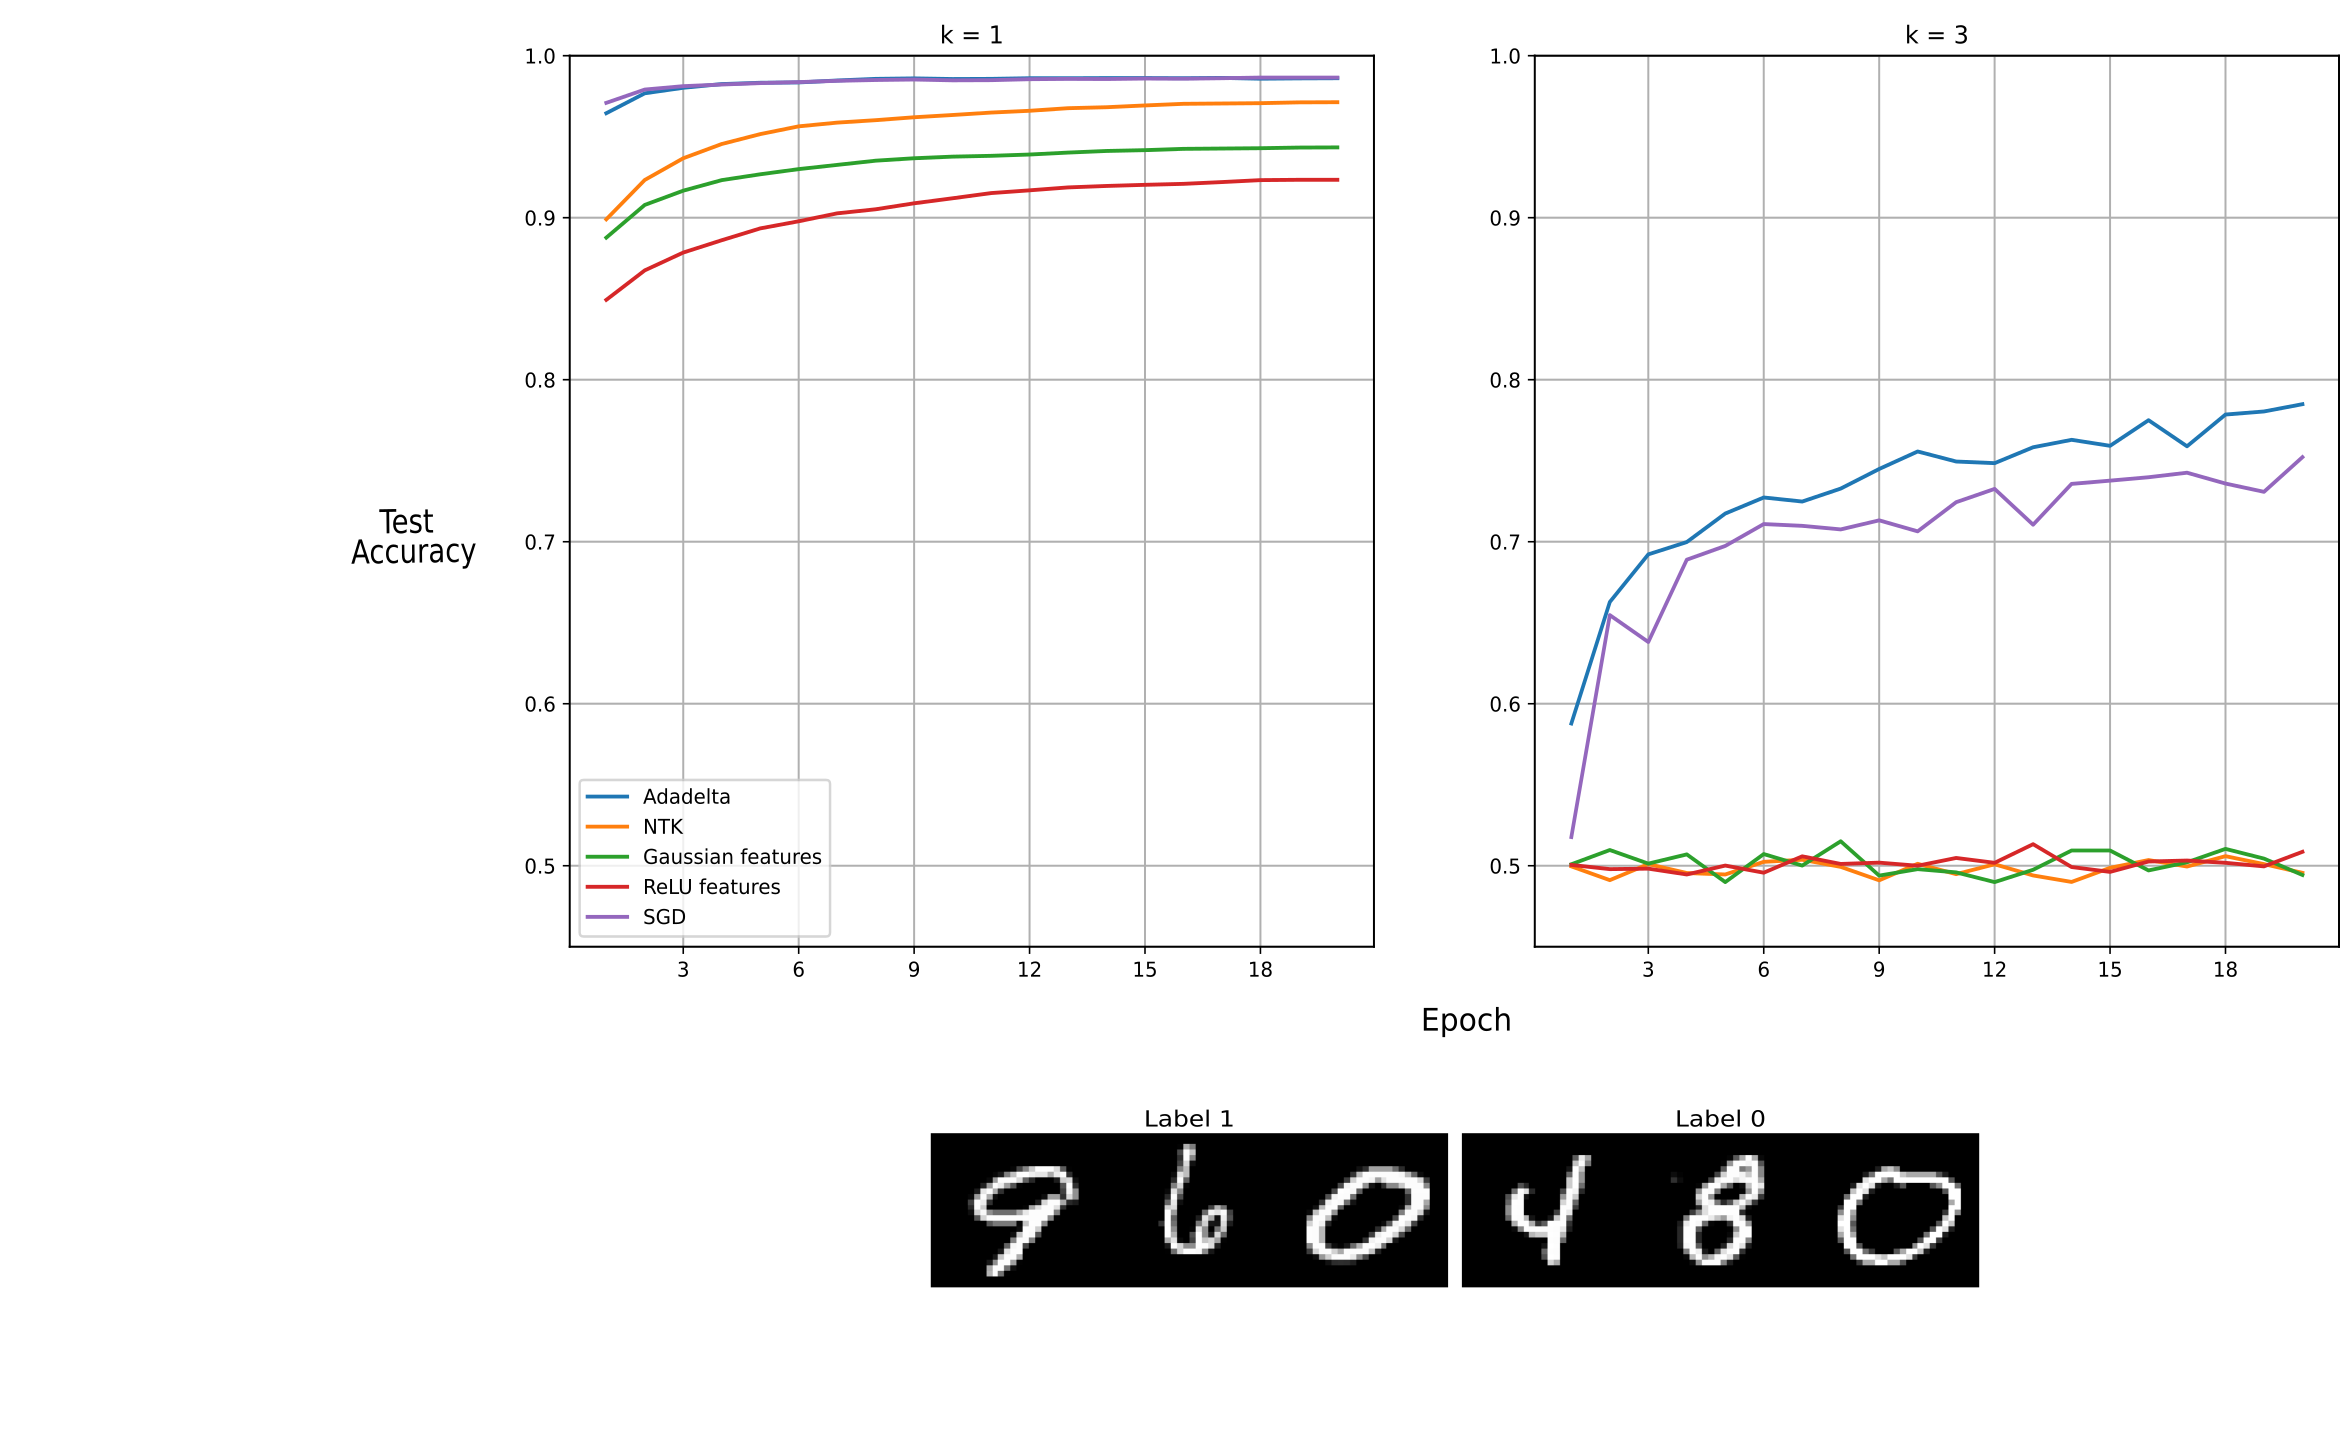
\includegraphics[width=1\linewidth]{figures/reproduce} 

}

\caption{Reproduced MNIST Parity Experiment Result \cite{DBLP:journals/corr/abs-2002-07400}}\label{fig:MNISTparity}
\end{figure}

\noindent The reproduced result can be observed in figure \ref{fig:MNISTparity}. Similar to results from \cite{DBLP:journals/corr/abs-2002-07400}, all the methods succeed learning for \(k=1\) case. However, adadelta and SGD slightly outperformed lazy methods in this setting. In the case of \(k=3\), adadelta and SGD almost reach \(80\%\), but the performance of lazy methods doesn't go beyond a random guess.~
After having the concrete picture from the previous study, it is intriguing to see how DFA would perform with SGD and adaptive methods on this particular problem. We will investigate it in chapter \ref{chap:chapter_3} with other experiments.

\hypertarget{random-data-problem}{%
\section{Random Data Problem}\label{random-data-problem}}

\textbf{TODO}: Explain why we need another problem (To test DFA capabilities on a different and challenging problem which has similar behaviour as parity - not learnable by some models-). Write how this data is generated.

\hypertarget{chap:chapter_3}{%
\chapter{Experiments}\label{chap:chapter_3}}

\minitoc

\noindent After having the previous study results, we can continue to test DFA on the parity learning problem. Train phase and the hyperparameter tuning process are explained in chapter \ref{chap:chapter_2}. These processes are the same for the following experiments. For all experiments, scratch implementations are used with minimal Pytorch functionalities. They are performed three times and plotted with their mean and standard deviation or with their confidence interval.\\
The same architectures are used as the previous study for BP and DFA, meaning that we have only a hidden layer with 512 neurons, and reLU is used as a non-linear function for the hidden layer. BCE is chosen as a loss function and, sigmoid is preferred for the non-linearity of the last layer. Networks are trained for twenty epochs unless others are specified, and at each epoch, train and test datasets are recreated as it is explained in chapter \ref{chap:chapter_2}. Weights of the networks are initialized uniformly with \(\frac{1}{\sqrt{input dim}}\) as in default Pytorch weight initialization. Moreover, the random matrix \(B\) is initialized with the same way to have similar behaviors as the weight matrix unless other specified.

\hypertarget{parity-learning-experiments}{%
\section{Parity Learning Experiments}\label{parity-learning-experiments}}

Since the experiment details are clear now, it is time to test DFA on parity learning problem with BP by using SGD.

\begin{figure}

{\centering 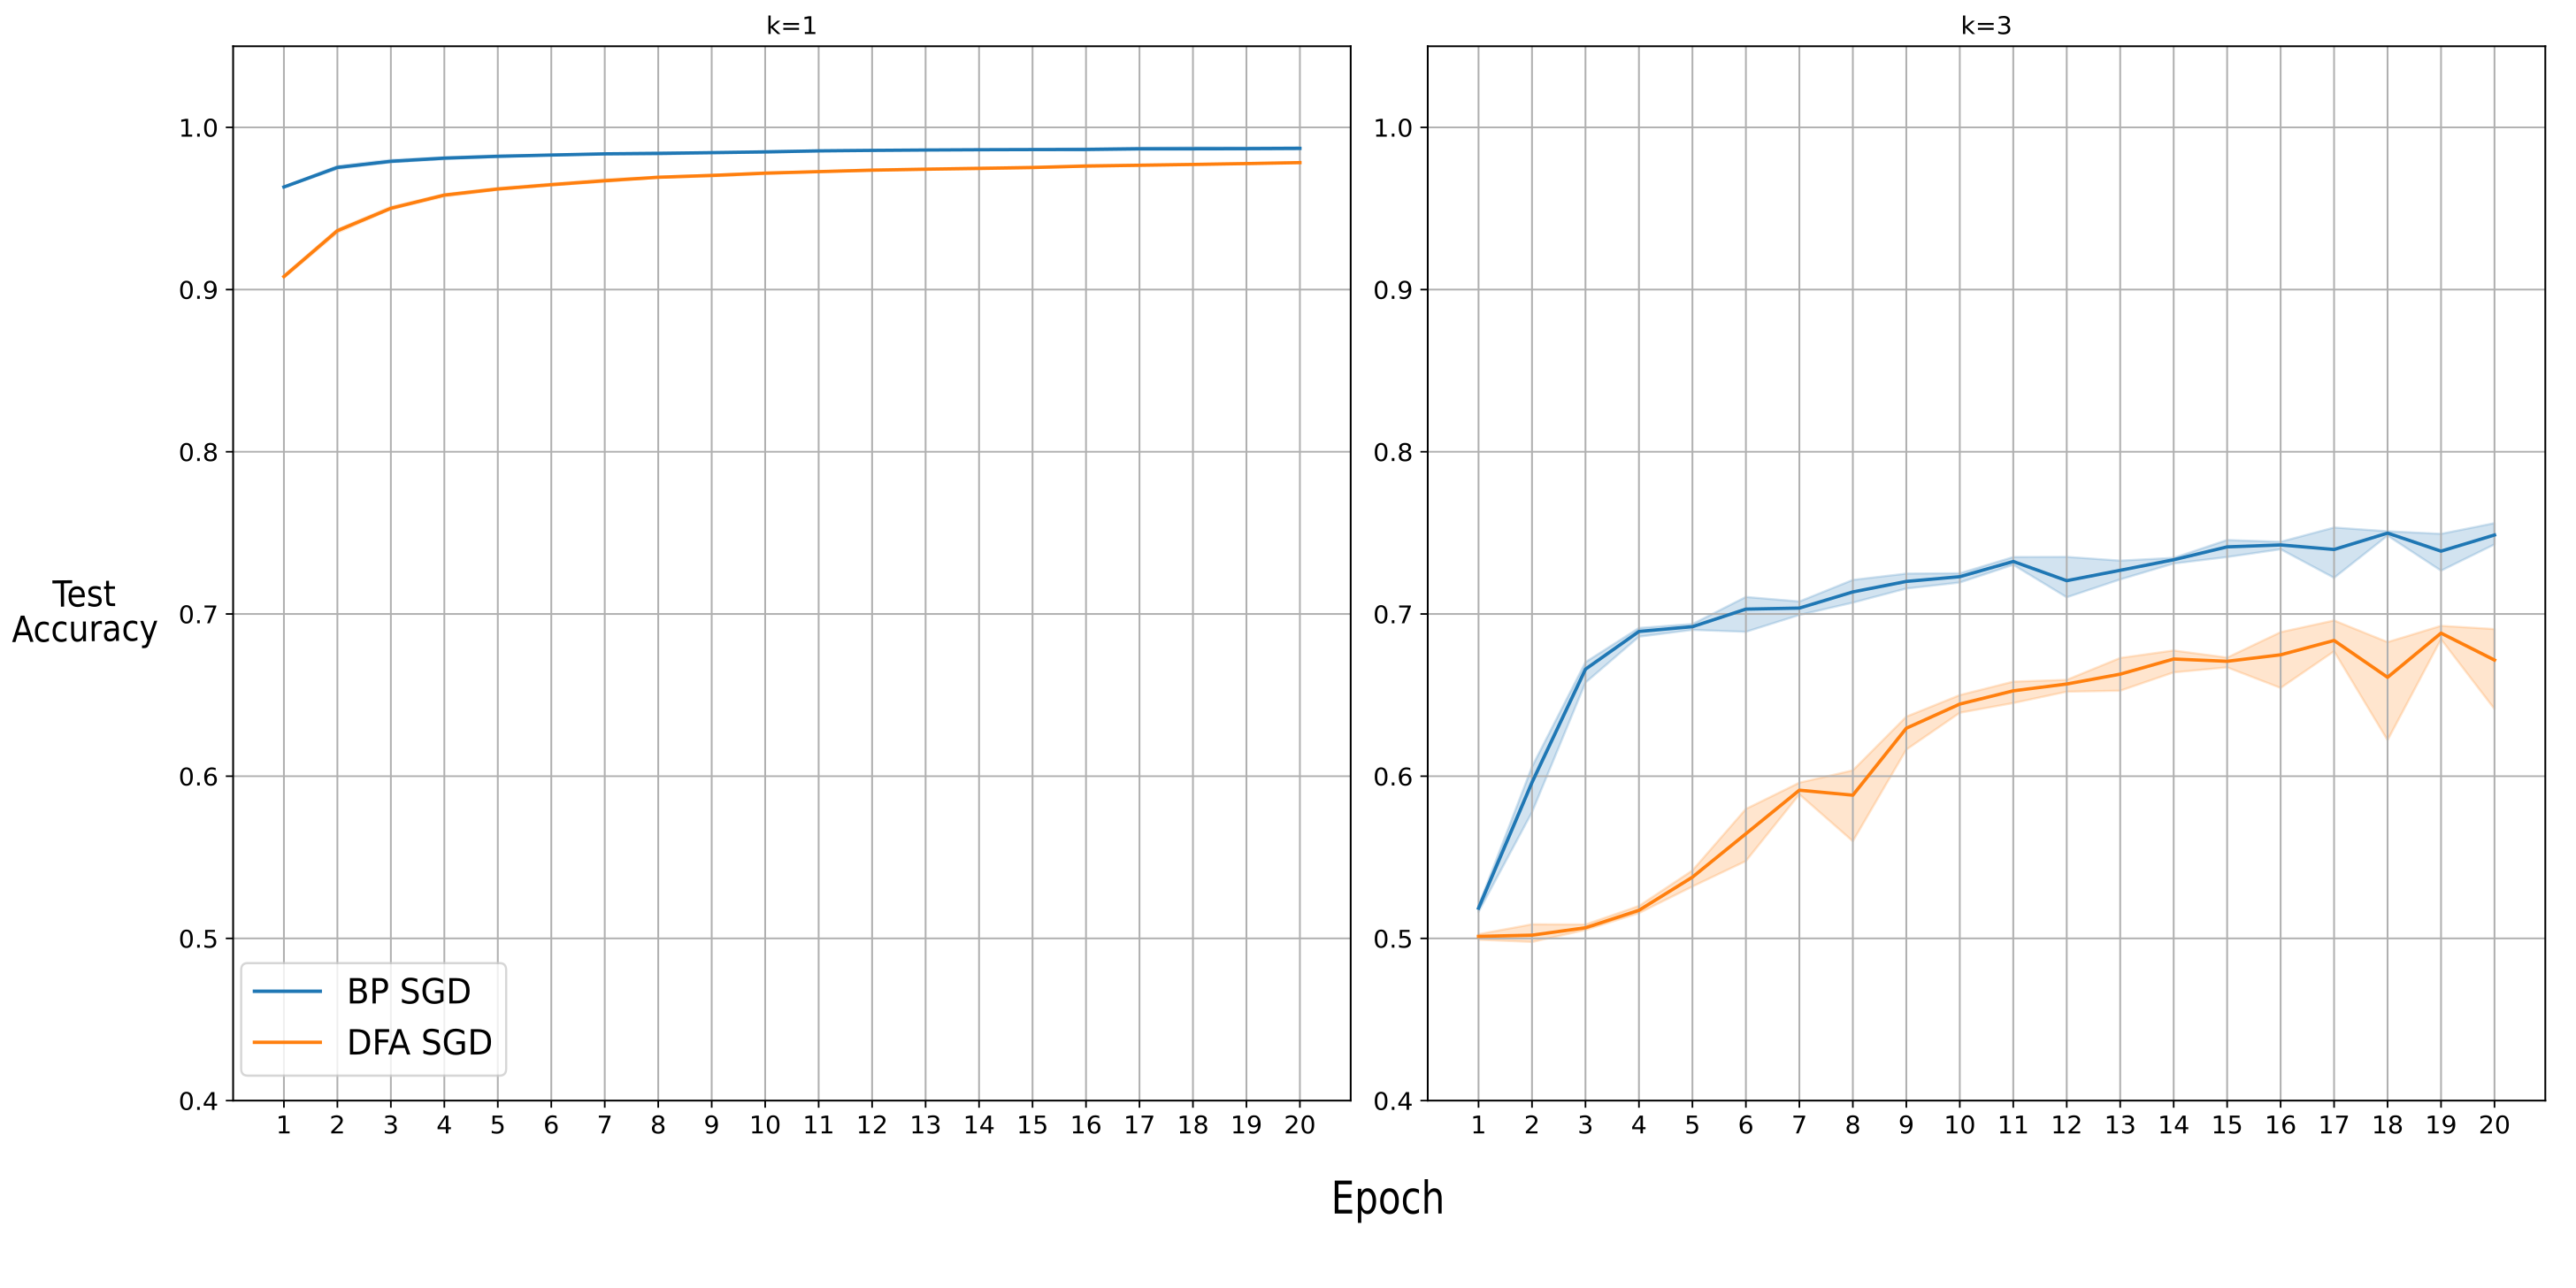
\includegraphics[width=1\linewidth]{figures/BPvsDFA_SGD} 

}

\caption{BP and DFA on Parity Problem with SGD}\label{fig:BPvsDFA}
\end{figure}

\noindent We can observe the results in \ref{fig:BPvsDFA} with \(95\%\) confidence interval. In the case \(k=1\), although DFA outperforms the lazy methods, it is behind the BP. In the case \(k=3\), it is obvious that DFA performs much better than lazy methods. However, the gap between BP and DFA is a bit higher than \(k=1\) case. It seems like there is a limit for DFA to reach with SGD that is \(\%70\). The reason is that DFA has an additional task to accomplish, which is aligning with BP's teaching signals. In other words, the network loses time while trying to make teaching signals useful. This delays the convergence and causes performance lag. We can see that during the first iterations, DFA does not converge fast enough to catch up with BP, and it always stays behind the BP.\\
The thrilling question is, is there a performance limit for DFA to reach, and can we get similar performance as BP by making some changes? For answering the first question, it is better to run DFA for more epochs to see if it can reach a similar performance as BP. Because with longer training, DFA will have time to align and converge. It would be convenient to test DFA with different random matrices to observe any improvement for the second question. Because it is clear that learning in DFA is strongly dependent on random matrix. Besides, it is interesting to test if DFA can learn with a different types of random matrices. During the learning rate phase of DFA, we noticed that it is susceptible to the learning rate. Having a small learning rate caused no convergence, and larger learning rates showed over-fitting within specified epoch numbers. Therefore we can use adaptive methods to have better convergence properties both in BP and DFA because these methods are specifically good at adjusting the learning rate, which is more difficult to tune for DFA than BP.\\
\noindent We trained DFA for 50 epochs with a tuned learning rate to observe if it can reach a similar performance as BP. At the same time, alignment between the random matrix and the transpose of the weight matrix is plotted. This alignment is measured by using the cosine similarity.

\begin{figure}

{\centering 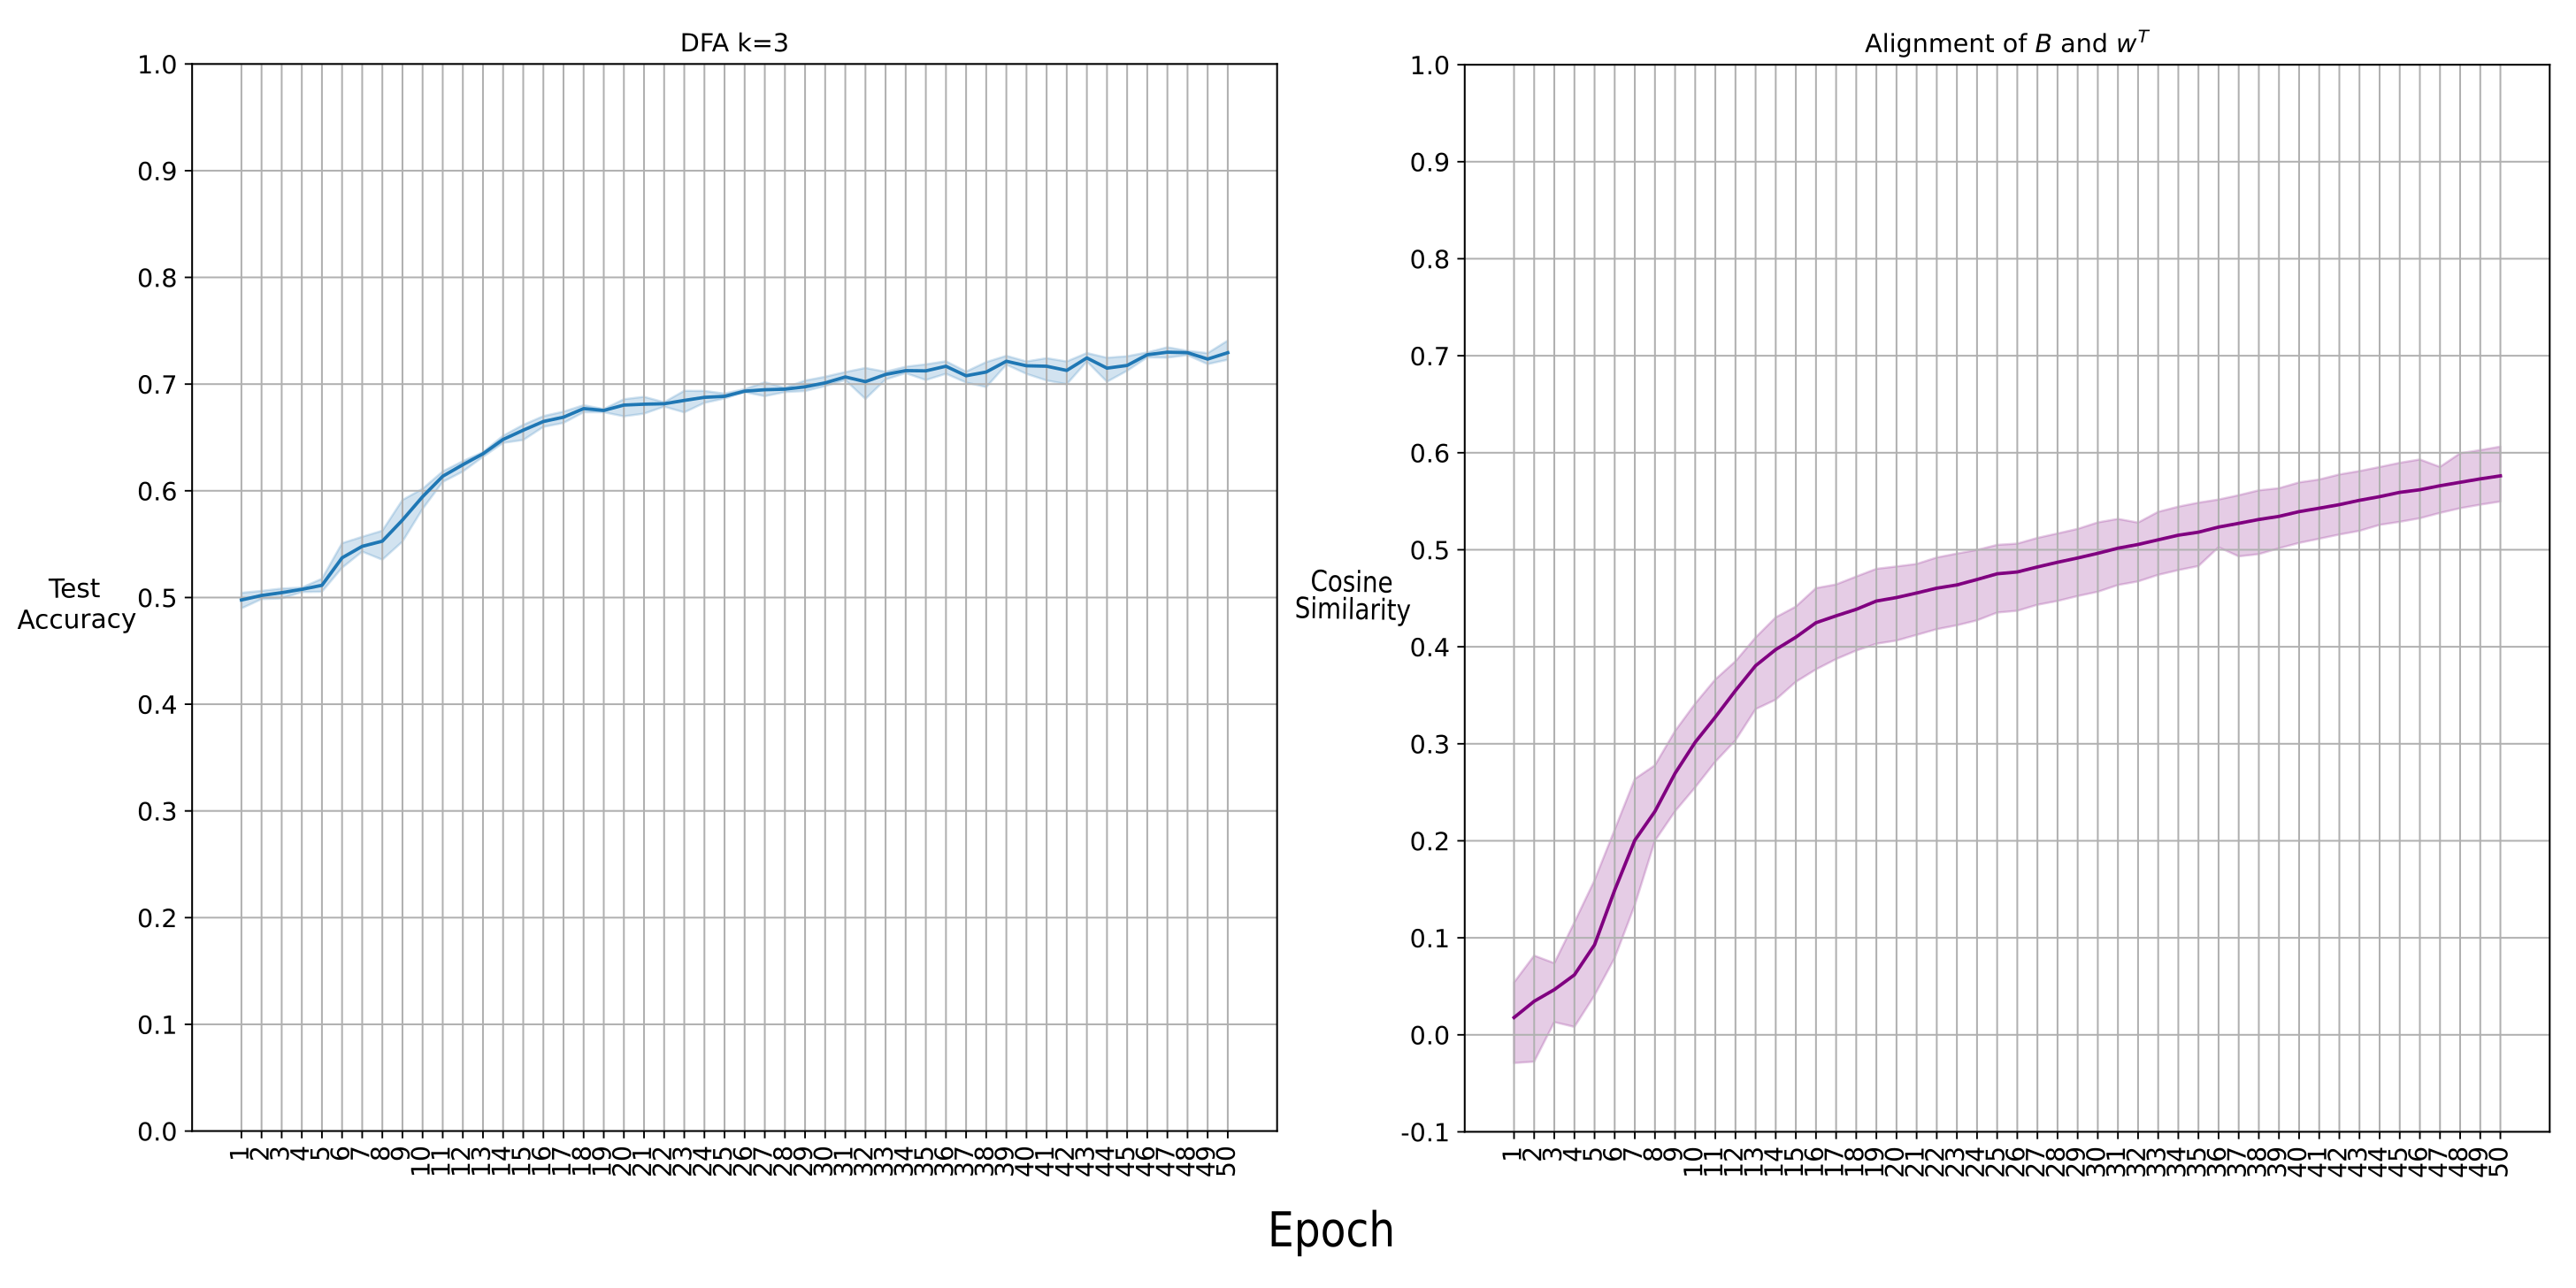
\includegraphics[width=1\linewidth]{figures/DFA_50epochs} 

}

\caption{DFA on Parity Problem with Alignment}\label{fig:DFA50epochs}
\end{figure}

\noindent From figure \ref{fig:DFA50epochs}, we can see that DFA can reach a similar performance as BP trained with SGD. This result approves our comments about the additional task DFA has and why it takes longer to achieve the same performance. On the right side of the plot, we can examine the alignment between the random matrix and the transpose of the weight matrix. At the beginning of training, the similarity is low. However, with advancing steps, we can see that alignment becomes higher, similar to the performance. It shows that the network aligns with the BP's teaching signals. In other words, the network learns how to learn by using the random matrix.
\noindent After having a similar performance from DFA with SGD, it is intriguing to test if we can achieve similar performance within the same epoch number. For this purpose, the first improvement attempt will be related to random matrices. Using different random matrices may influence the performance of DFA. Some of them might align better with BP's teaching signals. On the other hand, it is interesting to observe if we can learn with any random matrix.\\
Among uniform random matrix, three different random matrices are tested. They are initialized as the following: \textbf{standard uniform} is default Pytorch initialization that is uniformly distributed from \(0\) to \(1\). \textbf{Gaussian} is initialized normally with \(\mu\) and \(\sigma\) are equal to each other that is \(\frac{1}{\sqrt{input dim}}\). Lastly, \textbf{standard gaussian} is initialized with \(\mu=0\) and \(\sigma=1\).

\begin{figure}

{\centering 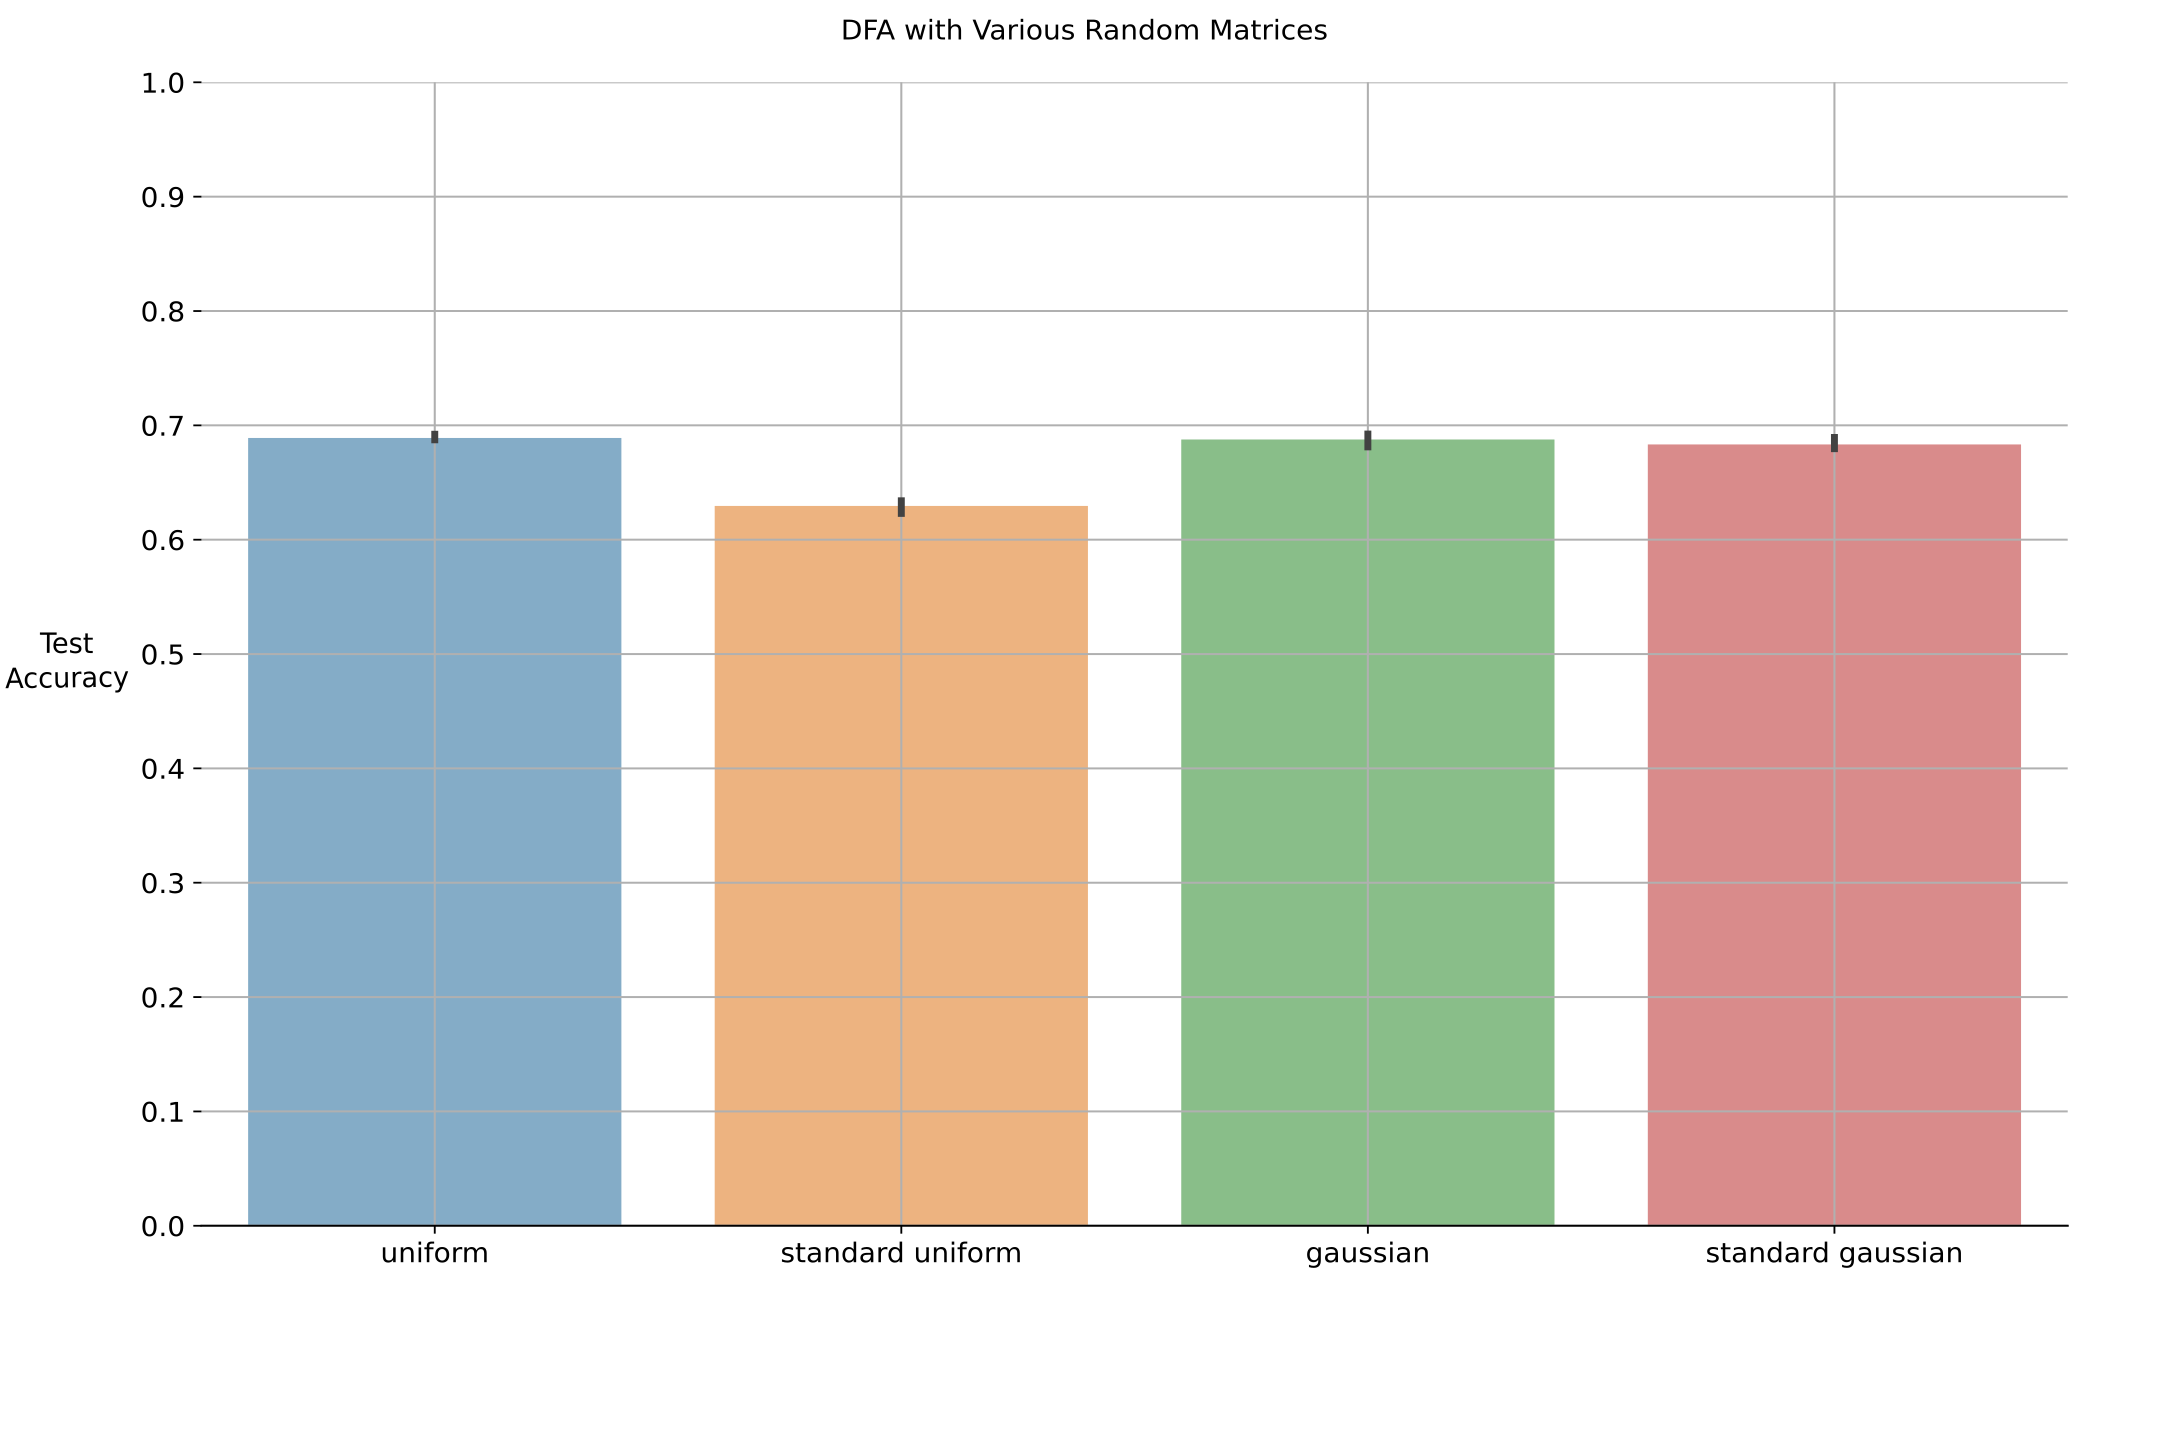
\includegraphics[width=1\linewidth]{figures/DFARandomMatrices} 

}

\caption{DFA on Parity Problem with Various Random Matrices}\label{fig:DFARandomMatrices}
\end{figure}

\noindent From figure \ref{fig:DFARandomMatrices}, we can observe that DFA can learn with any random matrices. However, it is essential to specify that learning rates for each random matrix are tuned and drastically different. Apart from standard uniform, the rest of the random matrices achieved similar performances, but they are still behind the BP. However, thanks to these results, we can see that DFA is highly sensitive to the learning rate. Because during the tuning phase, small learning rates did not converge within the specified epoch number. On the other hand, high learning rates demonstrated overfitting. Therefore, since adaptive methods have better convergence properties, they may increase the performance of DFA as they did in BP. For the rest of the DFA experiments, the random matrix is uniformly initialized since there is no significant improvement with other initializations.\\
\noindent Following the previous deduction, various adaptive methods are tested on the parity learning problem for BP and DFA. Their learning rates are tuned, as it is explained in the previous chapter. For the experiments, they are run three times, and their final test accuracies are plotted. The results are presented in figure \ref{mainExperiment}.

\begin{figure}

{\centering 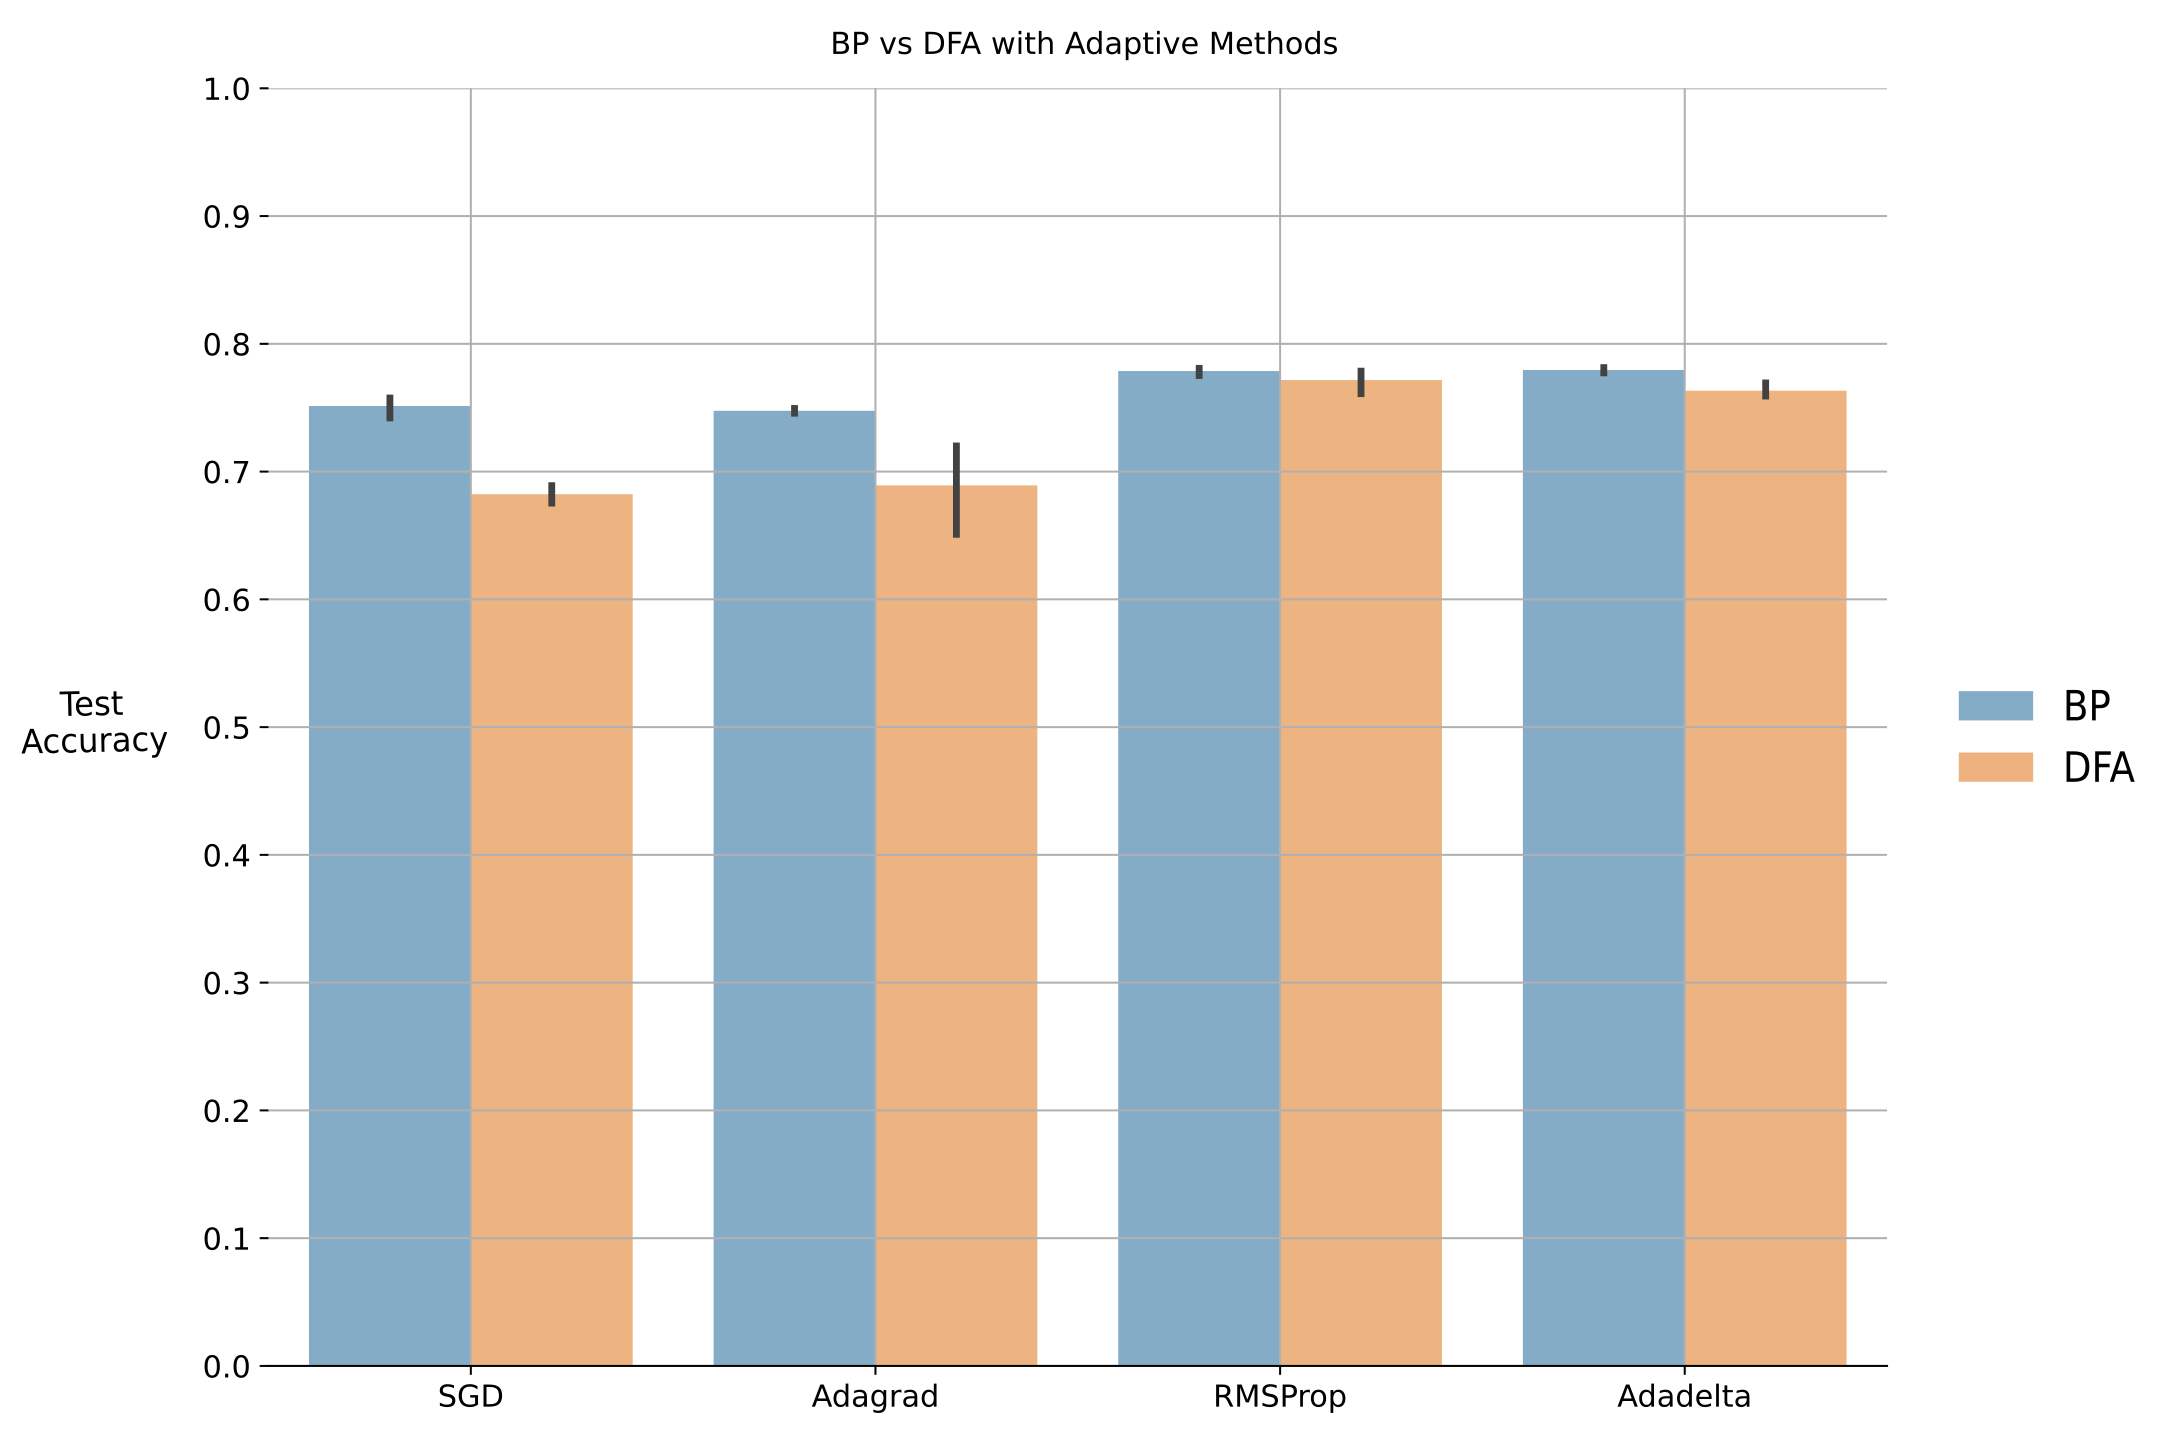
\includegraphics[width=1\linewidth]{figures/mainExperiment} 

}

\caption{DFA and BP on Parity Problem with Adaptive Methods}\label{fig:mainExperiment}
\end{figure}

\noindent As expected, adaptive methods improve the final test accuracy significantly for both BP and DFA. On average, DFA is still behind the BP, but with RMSProp and Adadelta, the gap is much smaller than with plain SGD. In other words, we can say that some adaptive methods help DFA more than BP with a higher standard deviation. With the last experiment, we could close the gap between BP and DFA on the parity learning problem thanks to adaptive methods.

\hypertarget{random-data-experiments}{%
\section{Random Data Experiments}\label{random-data-experiments}}

TODO: Report the random data experiments under this subtitle.

\hypertarget{conclusion}{%
\chapter*{Conclusion}\label{conclusion}}
\addcontentsline{toc}{chapter}{Conclusion}

TODO: Start summarizing all the process theoretical foundations, problems and wrap up the results of the experiments. Write some possible future studies. Write the take-home messages.

\startappendices

\hypertarget{chap:appendix_a}{%
\chapter{Backpropagation with Binary Cross-Entropy}\label{chap:appendix_a}}

Let's consider a simple binary classification task. It is common to use a network with a single logistic output with the binary cross-entropy loss function and for the sake of simplicity, let's assume that there is only one hidden layer.
\[
\begin{aligned}
BCE=-\sum_{i=1}^{n o u t}\left(y_i \log \left(\hat{y}_i \right)+\left(1-y_i\right) \log \left(1-\hat{y}_i\right)\right)
\end{aligned}
\]

Where \(y\) is the ground truth and \(\hat{y}\) is the output of the network. After having the loss function, let's continue with the forward pass.

\[
\begin{aligned} 
a_{k} &= h_{k-1} w_{k} + b_k \\
h_k &= f(a_{k})
\end{aligned}
\]

Where, \(w_k\) is the weight, \(b_{k}\) is the bias term, \(h_k\) is the output of the layer (which means that \(h_0 = X\) and \(h_2 = \hat{y}\)) and f is the non linear function. Please note that for last layer logistic function is used whereas for hidden layer reLU is used as non linear functions.\\
We can compute the derivative of the weights by using the chain rule.

\[
\begin{aligned} 
\frac{\partial BCE}{\partial w_{2}}=\frac{\partial BCE}{\partial \hat{y}} \frac{\partial \hat{y}}{\partial a_{2}} \frac{\partial a_{2}}{\partial w_{2}}
\end{aligned}
\]

Computing each factor in the term, we have:
\[
\begin{aligned}
\frac{\partial BCE}{\partial \hat{y}} &=\frac{-y}{\hat{y}}+\frac{1-y}{1-\hat{y}} \\
&=\frac{\hat{y}-y}{\hat{y}\left(1-\hat{y}\right)} \\
\frac{\partial \hat{y}}{\partial a_{2}} &=\hat{y}\left(1-\hat{y}\right) \\
\frac{\partial a_{2}}{\partial w_{2}} &=h_{1}^T
\end{aligned}
\]
This gives us:
\[
\frac{\partial BCE}{\partial w_{2}}=h_{1}^T\left(\hat{y}-y\right)
\]
We can calculate the derivative of the \(w_1\) concerning loss function as the following:

\[
\begin{aligned} 
\frac{\partial BCE}{\partial w_{1}}=\frac{\partial BCE}{\partial h_1} \frac{\partial h_1}{\partial a_{1}} \frac{\partial a_{1}}{\partial w_{1}}
\end{aligned}
\]
Compute each factor in the term again, we have:

\[
\begin{aligned}
\frac{\partial BCE}{\partial h_1} &= \frac{\partial BCE}{\partial \hat{y}} \frac{\partial \hat{y}}{\partial a_{2}} \frac{\partial a_{2}}{\partial h_{1}}  \\
&= \left(\hat{y}-y\right) w_{2}^T \\
\frac{\partial h_1}{\partial a_{1}} &=f'(a_1) \\
\frac{\partial a_{1}}{\partial h_{1}} &=X^T
\end{aligned}
\]
This gives us:
\[
\begin{aligned}
\frac{\partial BCE}{\partial w_{1}}= \left(X\right)^T\left(\hat{y}-y\right)\left(w_{2}^T\right) \odot f'(a_1)
\end{aligned}
\]
Where \(\odot\) is element-wise multiplication, similarly, bias terms can be calculated by following:

\[
\begin{aligned} 
\frac{\partial BCE}{\partial b_{2}}&=\frac{\partial BCE}{\partial \hat{y}} \frac{\partial \hat{y}}{\partial a_{2}} \frac{\partial a_{2}}{\partial b_{2}} \\
&= \left(\hat{y}-y\right)
\end{aligned}
\]

\[
\begin{aligned} 
\frac{\partial BCE}{\partial b_{1}}&=\frac{\partial BCE}{\partial h_1} \frac{\partial h_1}{\partial a_{1}} \frac{\partial a_{1}}{\partial b_{1}} \\
&= \left(\hat{y}-y\right)\left(w_{2}^T\right) \odot f'(a_1)
\end{aligned}
\]
After having all these results, we can update the parameters (weights and biases) using gradient descent and its variants.

\hypertarget{hidden-representation-of-digits-in-parity-problem}{%
\chapter{Hidden Representation of Digits in Parity Problem}\label{hidden-representation-of-digits-in-parity-problem}}

One of the interesting questions is: Does the network learn the digits individually when we train the network and make the necessary processes (summation, division), or does it memorize the way data is fed? We can answer this question by observing the hidden representation. If the network learns the digits well, we need to watch a good separation like the MNIST task. For this purpose, hidden representations of the networks trained with BP and DFA are plotted in two-dimensional space by using t-SNE \cite{vanDerMaaten2008} implementation of sklearn \cite{scikit-learn}.\\
The hidden representation of a single image in \(k=3\) case is obtained in the following way; we know that after we flatten the images, particular parts of each image are multiplied by corresponding parts of the weight matrix. Getting these parts and performing multiplication for each digit will give us the hidden representation of the individual digit trained in \(k=3\) case. Process is visualized in \ref{fig:HiddenRepProcess}. Since the t-SNE is a computationally expensive process, only 7500 random samples are plotted from the dataset.

\begin{figure}

{\centering 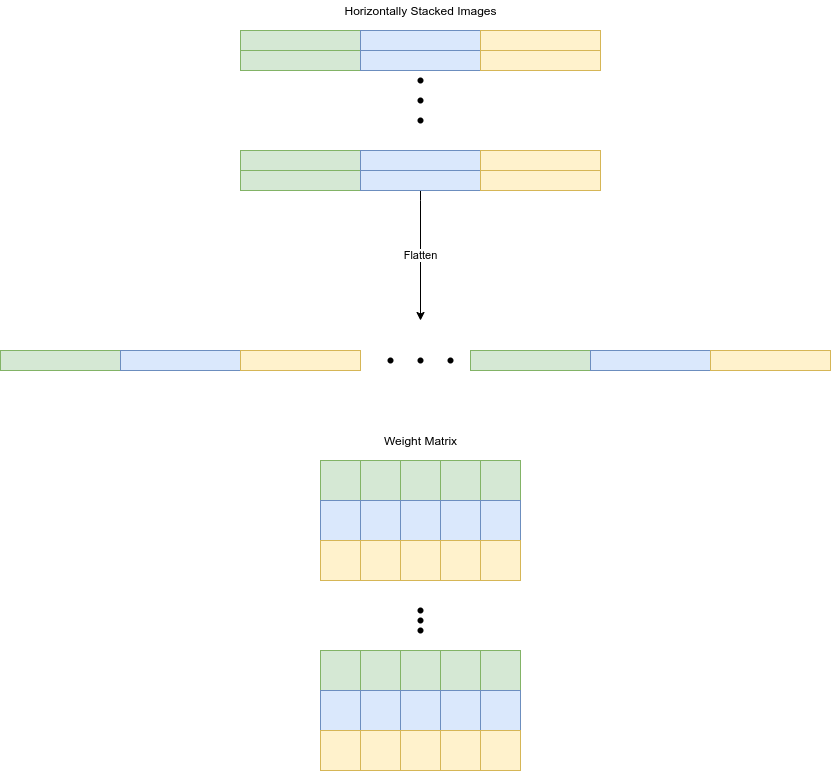
\includegraphics[width=0.6\linewidth]{figures/hidden_rep_process} 

}

\caption{Process of Hidden Representation}\label{fig:HiddenRepProcess}
\end{figure}

\noindent With this matrix multiplication, we have the hidden representation of each image. The rest is visualizing them by using the t-SNE. In figure \ref{fig:tSNEBPDFA} we can observe the results in two dimensions and say that the networks don't capture the information about the digits individually. They learn by memorizing the samples, not the digits.

\begin{figure}

{\centering 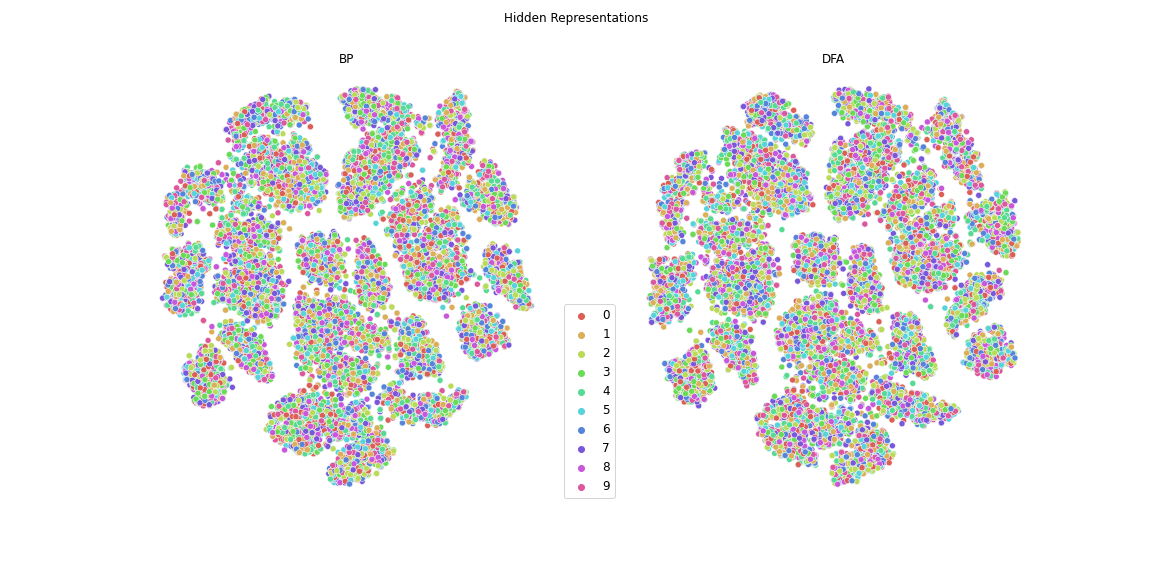
\includegraphics[width=1\linewidth]{figures/tsne_BPDFA} 

}

\caption{Hidden Representation of Digits in BP and DFA}\label{fig:tSNEBPDFA}
\end{figure}

\hypertarget{reproducibility}{%
\chapter{Reproducibility}\label{reproducibility}}

TODO: Write down the library versions, refer to the Github repository for the experiments, give information about the hardware. Explain the stochastic behavior of data.


%%%%% REFERENCES
\setlength{\baselineskip}{0pt} % JEM: Single-space References

{\renewcommand*\MakeUppercase[1]{#1}%
\printbibliography[heading=bibintoc,title={\bibtitle}]}


\end{document}
